%=================================================================
\documentclass[informatics,article,submit,pdftex,moreauthors]{Definitions/mdpi} 
% Changed from bdcc to informatics
%=================================================================
% Add packages and commands here.
\usepackage{booktabs} % For professional quality tables
\usepackage{multirow} % For multi-row cells in tables
\usepackage{siunitx} % For aligning numbers in tables
\usepackage{textcomp} % For better text symbols
\usepackage{adjustbox} % To fit tables to text width
\usepackage{tabularx} % For tables with adjustable-width columns

%=================================================================
\firstpage{1} 
\makeatletter 
\setcounter{page}{\@firstpage} 
\makeatother
\pubvolume{1}
\issuenum{1}
\articlenumber{0}
\pubyear{2025}
\copyrightyear{2025}
\datereceived{ } 
\daterevised{ }
\dateaccepted{ } 
\datepublished{ } 
%\hreflink{https://doi.org/}

%=================================================================
% Full title of the paper (Capitalized)
\Title{Systematic Fine-Tuning of Transformer Models for Domain-Specific Misinformation Detection in Spanish Social Media Text}

% MDPI internal command: Title for citation in the left column
%\TitleCitation{Systematic Fine-Tuning of Transformer Models for Domain-Specific Misinformation Detection in Spanish Social Media Text}

% Author Orchid ID
\newcommand{\orcidauthorA}{0009-0002-5686-1822} % Gabriel Hurtado Avilés (Placeholder)
\newcommand{\orcidauthorB}{0000-0003-2111-4982} % José Alejandro Reyes Ortiz (Placeholder)
\newcommand{\orcidauthorC}{0000-0002-2112-7049} % Román Anselmo Mora Gutiérrez (Placeholder)
\newcommand{\orcidauthorD}{0000-0002-3156-3231} % Josué Padilla Cuevas (Placeholder)
\newcommand{\orcidauthorE}{0000-0002-7488-0333} % Óscar Herrera Alcántara (Placeholder)

% Authors, for the paper
\Author{Gabriel Hurtado Avilés $^{1}$\orcidA{}, José A. Reyes-Ortiz $^{1}$*\orcidB{}, Román A. Mora-Gutiérrez $^{1}$\orcidC{}, Josué Padilla Cuevas $^{1}$\orcidD{} and Óscar Herrera Alcántara $^{1}$\orcidE{}}

% MDPI internal command: Authors, for metadata in PDF
\AuthorNames{Gabriel Hurtado Avilés, José Alejandro Reyes Ortiz, Román Anselmo Mora Gutiérrez, Josué Padilla Cuevas, and Óscar Herrera Alcántara}

% MDPI internal command: Authors, for citation in the left column
%\AuthorCitation{Hurtado Avilés, G.; Reyes-Ortiz, J.A.; Mora-Gutiérrez, R.A.; Padilla Cuevas, J.}

% Affiliations / Addresses
\address{%
$^{1}$ \quad Department of Systems, Autonomous Metropolitan University (UAM), Azcapotzalco Unit, Mexico City 02200, Mexico; gabrielhuav@gmail.com (G.H.A.); jaro@azc.uam.mx (J.A.R.-O.); mgra@azc.uam.mx (R.A.M.-G.); jpc@azc.uam.mx (J.P.C.); oha@azc.uam.mx (Ó.H.A.)}

% Contact information of the corresponding author
\corres{Correspondence: jaro@azc.uam.mx (J.A.R.-O.)}

%=================================================================
% Abstract
\abstract{While social media platforms are primary vectors for misinformation, automated detection systems remain largely confined to English. This paper presents a transferable, three-stage framework for fine-tuning transformer models to detect domain-specific deceptive content in Spanish. The pipeline comprises: (1) corpus unification, merging fragmented datasets into a 61,674-article resource mapped into three classes (Real, Fake, Satire) to prevent stylistic confounding; (2) systematic model optimization, extensively benchmarking classical metaheuristics against eight transformer architectures (including mBERT, XLM-RoBERTa, and BETO) using aggressive regularization to prevent overfitting; and (3) production deployment, encapsulating the optimized model as a containerized web application for real-time inference. Through rigorous experimentation, the Spanish-specific BETO encoder emerged as the state-of-the-art for this task, achieving an 89.18\% overall accuracy and a near-perfect 1.00 F1-score in isolating satire from malicious fake news. Adversarial robustness tests—utilizing named entity masking and typo injection—provide evidence that the model relies on deep semantic patterns rather than mere entity memorization, with satirical content retaining a 0.96 F1-score even under severe text degradation. The methodology is designed to be adaptable across domains: by substituting the training corpus, the same framework may in principle be retargeted to other digital threats, such as investment scams and phishing, provided that suitable labeled corpora are constructed and validated for each new domain. The complete framework, dataset, and application are open-source to support reproducible research and practical digital self-defense.}

% Keywords
\keyword{misinformation detection; transformer fine-tuning; social media analysis; domain-specific NLP; systematic regularization; BETO; transferable framework; Spanish fake news; web application deployment}

%%%%%%%%%%%%%%%%%%%%%%%%%%%%%%%%%%%%%%%%%%

\begin{document}

%%%%%%%%%%%%%%%%%%%%%%%%%%%%%%%%%%%%%%%%%%
\section{Introduction}
The proliferation of deceptive content on social media platforms represents one of the most pressing challenges at the intersection of machine learning and digital society \citep{bondielli2019survey}. The rapid expansion of social networks has transformed how information is created, disseminated, and consumed, creating unprecedented opportunities for the spread of misinformation, fraudulent schemes, and manipulative content.  This phenomenon disproportionately affects vulnerable demographics with limited media literacy skills \citep{higdon2022agree, higdon2025constructive}, undermining public trust in journalism, distorting democratic processes, and threatening public health outcomes \citep{tsfati2020causes, allcott2017social}. Critically, the problem extends far beyond traditional fake news: social media platforms are increasingly exploited for investment scams—such as pages impersonating state-owned enterprises with fabricated profit schemes \citep{scam2025investment}—fraudulent e-commerce impersonations featuring fake testimonials and artificial urgency \citep{scam2025cosmetics, scam2025ecommerce}, and an alarming proliferation of fake storefronts impersonating major retail chains with fabricated liquidation sales \citep{scam2026aurrera1, scam2026aurrera2, scam2026aurrera3, scam2026celulares}. Celebrity health misinformation—such as pages exploiting public figures' names to promote fraudulent medical products \citep{scam2025health}—further compounds the problem.  These diverse forms of digital deception disproportionately target elderly and digitally illiterate populations, and their sheer volume on social media feeds underscores the urgent need for automated, scalable detection systems.

While transformer-based models have achieved state-of-the-art performance in English-language misinformation detection \citep{kaliyar2021fakebert, singh2024comprehensive, rout2025reliable}, a fundamental methodological gap persists: the absence of systematic, reproducible frameworks for adapting these general-purpose models to \textit{domain-specific} deceptive content detection tasks. Most existing studies focus on reporting end-task accuracy without providing a transferable methodology that practitioners can apply to new domains, languages, or content types \citep{alghamdi2024comprehensive}. This gap is particularly acute for non-English languages and for emerging forms of social media fraud that lack established benchmark datasets.

The field of automated deceptive content detection has evolved through distinct methodological paradigms, reflecting advances in machine learning and natural language processing.  Early research in the 2010s relied on classical machine learning approaches—Support Vector Machines (SVMs), Naïve Bayes, Random Forests—combined with hand-crafted linguistic features such as Term Frequency-Inverse Document Frequency (TF-IDF) and Bag-of-Words (BoW) representations \citep{shu2017fake, ali2022fake, perez2018automatic}. While computationally efficient, these methods struggled to capture semantic nuances, sarcasm, and contextual meaning, limiting their effectiveness against sophisticated misinformation tactics. 

The mid-2010s witnessed a paradigm shift toward deep learning architectures.  Convolutional Neural Networks (CNNs) and Recurrent Neural Networks (RNNs) enabled automatic feature extraction from text, eliminating the need for manual feature engineering \citep{nasir2021fake, zhou2020survey}. However, these models were constrained by their inability to process long-range dependencies and bidirectional context effectively. 

The introduction of transformer architectures—particularly BERT \citep{devlin2018bert} and its variants—revolutionized the field by capturing bidirectional contextual representations through self-attention mechanisms \citep{vaswani2017attention}. Recent surveys \citep{singh2024comprehensive, alghamdi2024comprehensive} have documented the superiority of transformer-based approaches across multiple languages, with models such as FakeBERT \citep{kaliyar2021fakebert} leveraging datasets like LIAR \citep{wang2017liar} and FakeNewsNet alongside techniques including emotion-aware multitask learning \citep{choudhry2024emotion} and hybrid CNN-RNN architectures \citep{nasir2021fake}. 

However, despite these architectural advances, three interconnected challenges remain largely unaddressed in the literature. First, there is a \textbf{lack of systematic fine-tuning methodologies}: most studies report results from a narrow hyperparameter search without documenting the optimization trajectory or providing reproducible regularization strategies that can be transferred to new tasks \citep{blanco2024enhancing, martinez2021fake}. Second, there is a \textbf{scarcity of domain-specific resources for non-English languages}, particularly for Spanish—a language with over 500 million native speakers—where datasets are fragmented and incompatible \citep{singh2024comprehensive, posadas2019detection}. Third, a \textbf{persistent deployment gap} separates academic models from practical tools \citep{ali2022fake}: while papers report high accuracy, there is a striking absence of production-ready applications that communities can use for real-time verification.

This paper addresses these challenges by proposing a \textbf{systematic and transferable framework} for fine-tuning pretrained transformer models for domain-specific misinformation detection on social media. The framework is structured as a three-stage pipeline—corpus unification, systematic regularization, and production deployment—and is intended to be adaptable across domains: while validated here on Spanish-language fake news detection, the same methodology could in principle be applied to detect other forms of social media deception, such as investment scams (e.g., fraudulent cryptocurrency or petroleum investment pages), fake e-commerce sites impersonating legitimate retailers, and phishing campaigns, provided that appropriate labeled corpora are constructed for each target domain. We note that these additional domains are presented as motivating directions for future work rather than as empirically validated results in this study.

A progressive research design was adopted: a baseline is first established with classical NLP methods (TF-IDF representations optimized via five metaheuristic algorithms), followed by a fine-tuned transformer model whose systematic regularization methodology is documented in full.

The main contributions of this work are:
\begin{itemize}
    \item \textbf{A Transferable Fine-Tuning Framework:} A systematic three-stage pipeline (corpus unification, aggressive regularization, containerized deployment) is proposed for adapting pretrained transformer models to domain-specific deceptive content detection. The framework is explicitly designed to be transferable across languages, content domains, and social media platforms.
    \item \textbf{A Systematic Regularization and Early Stopping Methodology:} Through extensive experimentation across multiple architectures, we document a strong regularization strategy for fine-tuning the monolingual BETO encoder. The methodology achieved an 89.18\% overall accuracy and a 0.9095 Macro F1-Score on a challenging 3-class paradigm, with results reproduced across two independent deep learning frameworks. The training trajectories demonstrate how a dynamic early stopping mechanism, combined with this regularization regime, keeps the validation loss on a stable plateau and prevents the catastrophic overfitting commonly observed in high-capacity transformers, providing a reproducible recipe for practitioners facing similar optimization challenges.
    \item \textbf{A Unified Spanish Corpus:} A standardized corpus of 61,674 Spanish news articles was constructed from four academic datasets \citep{posadas2019detection, acosta2019construccion, tretiakov2022detection, blanco2024enhancing} enhanced with web-scraped satirical content, achieving a three-class distribution (35.3\% fake, 50.2\% real, 14.5\% satire)—one of the largest resources for this task.
    \item \textbf{A Production-Ready Web Application:} The optimized model was deployed as a Docker-containerized web application capable of real-time URL analysis, demonstrating that the framework extends beyond academic benchmarks to deliver practical tools for digital self-defense \citep{ali2022fake}.
\end{itemize}

The complete framework is publicly available to encourage reproducibility. By substituting the training corpus, the same pipeline could in principle be adapted to detect investment scams, phishing pages, fraudulent e-commerce sites, and other forms of social media deception; demonstrating this adaptability empirically on additional domains is a primary direction for future work.

%%%%%%%%%%%%%%%%%%%%%%%%%%%%%%%%%%%%%%%%%%
\section{Related Work: Detection Paradigms and Methodological Gaps}
The scholarly approach to deceptive content detection has evolved through several paradigms, shifting from socio-cognitive media literacy approaches to highly complex neural architectures. As summarized in Table \ref{tab:methodological_paradigms}, early computational efforts relied heavily on classical machine learning models utilizing static statistical features like TF-IDF. While these provided interpretable baselines, their inability to capture sequential semantic dependencies led to the adoption of deep learning architectures (CNNs and RNNs). Recently, transformer-based models have dominated the field by leveraging bidirectional self-attention to contextualize nuanced deceptive language. 


\begin{table}[H]
\centering
\caption{Comparison of Methodological Paradigms in Deceptive Content Detection on Social Media.}
\label{tab:methodological_paradigms}
\adjustbox{width=\textwidth,center}{%
\scriptsize
\begin{tabular}{lllll}
\toprule
\textbf{Paradigm} & \textbf{Core Principle} & \textbf{Key Studies} & \textbf{Strengths} & \textbf{Limitations} \\
\midrule
\begin{tabular}[t]{@{}l@{}}\textbf{Media Literacy}\\\textbf{\& Societal Impact}\end{tabular} & \begin{tabular}[t]{@{}l@{}}Address root causes\\through critical\\thinking education\end{tabular} & \begin{tabular}[t]{@{}l@{}}Higdon \citep{higdon2022agree},\\Higdon \citep{higdon2025constructive},\\Tsfati et al. \citep{tsfati2020causes}\end{tabular} & \begin{tabular}[t]{@{}l@{}}Addresses cultural\\and cognitive factors\end{tabular} & \begin{tabular}[t]{@{}l@{}}Does not provide\\automated detection\end{tabular} \\
\midrule
\begin{tabular}[t]{@{}l@{}}\textbf{Classical Machine}\\\textbf{Learning}\end{tabular} & \begin{tabular}[t]{@{}l@{}}Statistical features\\from text (TF-IDF, BoW)\end{tabular} & \begin{tabular}[t]{@{}l@{}}Shu et al. \citep{shu2017fake},\\Ali et al. \citep{ali2022fake},\\Thota et al. \citep{thota2018fake}\end{tabular} & \begin{tabular}[t]{@{}l@{}}Computationally\\efficient, interpretable\end{tabular} & \begin{tabular}[t]{@{}l@{}}Limited semantic\\understanding\end{tabular} \\
\midrule
\begin{tabular}[t]{@{}l@{}}\textbf{Deep Learning}\\\textbf{(CNN/RNN)}\end{tabular} & \begin{tabular}[t]{@{}l@{}}Automatic feature\\extraction via\\neural networks\end{tabular} & \begin{tabular}[t]{@{}l@{}}Nasir et al. \citep{nasir2021fake},\\Zhou \& Zafarani \citep{zhou2020survey}\end{tabular} & \begin{tabular}[t]{@{}l@{}}Better feature\\learning, reduced\\manual engineering\end{tabular} & \begin{tabular}[t]{@{}l@{}}Limited handling of\\long-range dependencies\end{tabular} \\
\midrule
\begin{tabular}[t]{@{}l@{}}\textbf{Transformers}\\\textbf{(BERT-based)}\end{tabular} & \begin{tabular}[t]{@{}l@{}}Bidirectional context\\via self-attention\\mechanisms\end{tabular} & \begin{tabular}[t]{@{}l@{}}Singh et al. \citep{singh2024comprehensive},\\Alghamdi et al. \citep{alghamdi2024comprehensive},\\Kaliyar et al. \citep{kaliyar2021fakebert},\\Rout et al. \citep{rout2025reliable}\end{tabular} & \begin{tabular}[t]{@{}l@{}}State-of-the-art\\performance, captures\\semantic nuances\end{tabular} & \begin{tabular}[t]{@{}l@{}}Computationally\\expensive, requires\\large datasets\end{tabular} \\
\midrule
\begin{tabular}[t]{@{}l@{}}\textbf{Multimodal \&}\\\textbf{Emotion-Aware}\end{tabular} & \begin{tabular}[t]{@{}l@{}}Integrates text, images,\\and emotional features\end{tabular} & \begin{tabular}[t]{@{}l@{}}Choudhry et al. \citep{choudhry2024emotion},\\Zhen \& Li \citep{zhen2026csteer},\\Shang et al. \citep{shang2025eticd}\end{tabular} & \begin{tabular}[t]{@{}l@{}}Holistic analysis,\\improved accuracy\end{tabular} & \begin{tabular}[t]{@{}l@{}}Complex architectures,\\limited Spanish resources\end{tabular} \\
\bottomrule
\end{tabular}
}
\end{table}

\subsection{Language Resources and the "Deployment Gap"}
A significant bottleneck for advancing deceptive content detection—whether fake news, scam pages, or fraudulent content—is the availability of large-scale, comprehensive datasets, particularly for languages other than English. Furthermore, a persistent issue in the academic NLP community is the ``deployment gap'': the divide between models achieving high accuracy in controlled research environments and the scarcity of practical, production-ready tools available to the public. 

\subsection{Systematic Fine-Tuning and State-of-the-Art Transformers}
While models like BERT and its multilingual variants achieve strong results in NLP tasks, they require careful hyperparameter tuning—a process rarely documented systematically in the literature. Recent comprehensive reviews \citep{singh2024comprehensive, alghamdi2024comprehensive} highlight that while hybrid and multimodal architectures exist, properly configured transformers \citep{rout2025reliable} remain the most robust approach for textual analysis. Specifically for the Spanish language, recent benchmarks emphasize the need to compare base multilingual models, such as mBERT \citep{devlin2018bert} and XLM-RoBERTa \citep{conneau2019unsupervised}, against language-specific encoders like BETO \citep{canete2020spanish} and RoBERTa-bne \citep{gutierrez2022roberta} to truly establish state-of-the-art performance \citep{blanco2024enhancing}. This approach of systematic hyperparameter optimization for BERT-based models in Spanish NLP tasks has also been demonstrated in the biomedical domain \citep{padilla2024medicobert}, further motivating the reproducible fine-tuning methodology proposed in this work.

To synthesize the current landscape and highlight the specific gaps addressed by this research, Tables \ref{tab:related_work_summary1} and \ref{tab:related_work_summary2} provide a comprehensive breakdown of recent key studies. Table \ref{tab:related_work_summary1} details approaches centered on corpus creation and transformer models, while Table \ref{tab:related_work_summary2} categorizes works utilizing metaheuristic and classical hybrid architectures.

\begin{table}[H]
\centering
\caption{Summary of key related works (Part 1): Corpus Creation \& Transformer Application for Deceptive Content Detection.}
\label{tab:related_work_summary1}
\adjustbox{width=\textwidth,center}{%
\small
\begin{tabular}{llll}
\toprule
\textbf{Author(s) [Ref.]} & \textbf{Contribution} & \textbf{Key Finding / Performance} & \textbf{Limitation Addressed by This Work} \\
\midrule
\begin{tabular}[t]{@{}l@{}}Posadas-Durán\\et al. \citep{posadas2019detection}\end{tabular} & \begin{tabular}[t]{@{}l@{}}Created a pioneering Spanish\\corpus (971 articles) with\\a stylometric focus.\end{tabular} & \begin{tabular}[t]{@{}l@{}}Established baseline\\stylometric markers for\\Spanish fake news.\end{tabular} & \begin{tabular}[t]{@{}l@{}}Corpus is too small for modern\\transformer fine-tuning.\end{tabular} \\
\midrule
\begin{tabular}[t]{@{}l@{}}Kaliyar et al. \citep{kaliyar2021fakebert}\end{tabular} & \begin{tabular}[t]{@{}l@{}}Proposed FakeBERT, a\\deep learning model combining\\BERT with CNN layers.\end{tabular} & \begin{tabular}[t]{@{}l@{}}Achieved 98.9\% accuracy\\on English datasets.\end{tabular} & \begin{tabular}[t]{@{}l@{}}Focused exclusively on\\English-language content.\end{tabular} \\
\midrule
\begin{tabular}[t]{@{}l@{}}Blanco-Fernández\\et al. \citep{blanco2024enhancing}\end{tabular} & \begin{tabular}[t]{@{}l@{}}Applied BERT/RoBERTa\\to a large, politically-focused\\dataset (57k articles).\end{tabular} & \begin{tabular}[t]{@{}l@{}}High accuracy, but limited\\by domain specificity.\end{tabular} & \begin{tabular}[t]{@{}l@{}}Lacked systematic regularization\\for out-of-domain transfer.\end{tabular} \\
\midrule
\begin{tabular}[t]{@{}l@{}}Martínez-Gallego\\et al. \citep{martinez2021fake}\end{tabular} & \begin{tabular}[t]{@{}l@{}}Explored different BERT\\variants (including BETO)\\for Spanish fake news\\detection.\end{tabular} & \begin{tabular}[t]{@{}l@{}}BETO outperformed\\multilingual variants in\\preliminary tests.\end{tabular} & \begin{tabular}[t]{@{}l@{}}No production-ready deployment\\or adversarial testing.\end{tabular} \\
\midrule
\begin{tabular}[t]{@{}l@{}}Rout et al. \citep{rout2025reliable}\end{tabular} & \begin{tabular}[t]{@{}l@{}}Proposed an enhanced\\attention-based transformer\\model for reliable fake\\news detection.\end{tabular} & \begin{tabular}[t]{@{}l@{}}Improved reliability\\and attention focus.\end{tabular} & \begin{tabular}[t]{@{}l@{}}Focused on English, without\\multi-class satire separation.\end{tabular} \\
\bottomrule
\end{tabular}
}
\end{table}

\begin{table}[H]
\centering
\caption{Summary of key related works (Part 2): Metaheuristic, Classical, and Hybrid Approaches.}
\label{tab:related_work_summary2}
\adjustbox{width=\textwidth,center}{%
\small
\begin{tabular}{llll}
\toprule
\textbf{Author(s) [Ref.]} & \textbf{Contribution} & \textbf{Key Finding / Performance} & \textbf{Limitation Addressed by This Work} \\
\midrule
\begin{tabular}[t]{@{}l@{}}Yildirim \citep{yildirim2023novel}\end{tabular} & \begin{tabular}[t]{@{}l@{}}Hybrid multi-thread metaheuristic\\approach for fake news detection.\end{tabular} & \begin{tabular}[t]{@{}l@{}}Improved optimization\\speed and feature selection.\end{tabular} & \begin{tabular}[t]{@{}l@{}}Classical models lack deep\\contextual semantic understanding.\end{tabular} \\
\midrule
\begin{tabular}[t]{@{}l@{}}Thota et al. \citep{thota2018fake}\end{tabular} & \begin{tabular}[t]{@{}l@{}}Early deep learning approach\\using traditional neural networks\\for fake news detection.\end{tabular} & \begin{tabular}[t]{@{}l@{}}Demonstrated NN superiority\\over classic ML classifiers.\end{tabular} & \begin{tabular}[t]{@{}l@{}}Pre-transformer era; lacks\\bidirectional attention.\end{tabular} \\
\midrule
\begin{tabular}[t]{@{}l@{}}Gravanis et al. \citep{gravanis2019behind}\end{tabular} & \begin{tabular}[t]{@{}l@{}}Systematic benchmarking of\\classical ML classifiers and\\feature representations.\end{tabular} & \begin{tabular}[t]{@{}l@{}}Linguistic cues provide\\strong baseline signals.\end{tabular} & \begin{tabular}[t]{@{}l@{}}Did not evaluate transferability\\to modern digital fraud domains.\end{tabular} \\
\bottomrule
\end{tabular}
}
\end{table}

\section{Materials and Methods}

The methodology is structured as a transferable three-stage pipeline for adapting pretrained transformers to domain-specific deceptive content detection. While validated on Spanish fake news, each stage is designed to be reusable and adaptable to other detection domains. As illustrated in Figure \ref{fig:metodologia_general_p1}, the pipeline comprises: (1) \textbf{Corpus Unification}—aggregating and balancing heterogeneous datasets; (2) \textbf{Systematic Model Optimization}—comparing classical and deep learning paradigms through a documented regularization trajectory; and (3) \textbf{Production Deployment}—containerizing the optimal model for real-time inference.

% Part 1 (Image)
\begin{figure}[H]
\centering

\includegraphics[width=\textwidth]{Figures/system_architecture_p1.png}
\caption{Overview of the proposed research methodology (Part 1/3): Data Unification and Processing.}
\label{fig:metodologia_general_p1}
\end{figure}

\subsection{Stage 1: Corpus Unification and Processing}
The first stage addresses a common challenge: constructing a unified dataset from fragmented sources. The unification methodology (schema standardization, content-based deduplication, targeted augmentation) is generalizable to any detection domain. A unified corpus was constructed by aggregating four publicly available datasets: the Spanish Fake News Corpus (572 articles) \citep{posadas2019detection}, the Acosta Dataset (598 articles) \citep{acosta2019construccion}, the Tretiakov Dataset (2,000 articles) \citep{tretiakov2022detection}, and the Spanish Political Dataset (57,231 articles) \citep{blanco2024enhancing}, yielding an initial pool of \textbf{60,401} articles. Table \ref{tab:comparacion_exhaustiva_corpus} details each source.

\begin{table}[H]
\centering
\caption{Exhaustive comparison of the characteristics of the corpora used in the construction of the unified dataset.}
\label{tab:comparacion_exhaustiva_corpus}
\adjustbox{width=\textwidth,center}{%
\scriptsize
\begin{tabular}{lccccc}
\toprule
\textbf{Comparative Aspect} & \textbf{Posadas-Durán} & \textbf{Acosta} & \textbf{Tretiakov} & \textbf{Blanco-Fernández} & \textbf{El Deforma} \\
\midrule
\textbf{Initial Corpus Size} & 572 articles & 598 articles & 2,000 articles & 57,231 articles & 8,985 articles \\
\textbf{Creation Year} & 2019-2021 & 2019 & 2022 & 2024 & 2025 (extraction) \\
\textbf{Methodological Focus} & Stylometric & NLP Baselines & Traditional ML & Transformers & Satirical Content \\
\textbf{Thematic Domain} & General & General & General & Political & Satirical/General \\
\textbf{Class Distribution} & Balanced & Balanced & Balanced & Balanced & Satire Only \\
\textbf{Contribution (Pre-Dedup)} & 0.95\% & 0.99\% & 3.31\% & 94.75\% & 14.6\% (added later) \\
\bottomrule
\end{tabular}
}
\end{table}

To ensure data quality and mitigate semantic overlaps that could cause data leakage, a robust deduplication protocol was implemented following the preprocessing guidelines established by Acosta \citep{acosta2019construccion}. Prior to deduplication, texts underwent normalization (lowercasing, removal of non-alphanumeric characters, and whitespace standardization). Content hashing on the normalized text identified and removed exactly \textbf{7,712} near-duplicates from the initial 60,401 collected records. This precise filtering yielded exactly \textbf{52,689} unique articles (21,746 fake and 30,943 real).

\textbf{Methodological Evolution: From Binary to Multiclass Classification.} 
Initially, the research design conceptualized a binary classification task (Real vs. Fake), incorporating satirical articles as part of the "Fake" class to address class imbalance. However, extensive literature and preliminary evaluations revealed a critical construct-validity vulnerability: satire relies on irony, exaggeration, and parody markers, whereas malicious fake news relies on deceptive imitation of journalistic tone. Conflating the two forces the model to learn source-specific humor rather than robust misinformation cues, leading to miscalibration.

To address this, the methodology evolved into a \textbf{three-class classification formulation}: FAKE (0), REAL (1), and SATIRE (2). The final, rigorously structured corpus consists of exactly \textbf{61,674 records}: the 52,689 deduplicated factual/deceptive articles, supplemented by an isolated class of \textbf{8,985} satirical articles extracted via web scraping from regional sources. This structural evolution and the resulting class distribution, which transitioned from a highly imbalanced binary setup to a three-class architecture, is visually summarized in Figure \ref{fig:corpus_balance}.

This three-class architecture ensures the model learns to explicitly distinguish malicious disinformation from legitimate creative parody.

Regarding sequence length, although the BERT-based architectures used here support up to 512 subword tokens, exploratory analysis showed that the most discriminative deceptive markers (e.g., clickbait headlines and urgency triggers in the opening sentences) are heavily concentrated at the beginning of each article. We therefore tokenized inputs to a maximum length of 128 tokens for all fine-tuning experiments, which substantially reduced memory and compute requirements while preserving the leading content most relevant to classification. This choice avoids the overhead of long-sequence encoders (such as Longformer or BigBird) for this specific domain. The 512-token capacity of the architecture is retained at inference time for robustness to longer inputs.

\begin{figure}[H]
\centering

\includegraphics[width=\linewidth]{Figures/corpus_balance.png}
\caption{Visual representation of the corpus unification process. The dataset was expanded by strategically adding 8,985 SATIRE articles via web scraping, resulting in a three-class final distribution: Fake (35.3\%), Real (50.2\%), and Satire (14.5\%). Source: Authors' own elaboration based on study data.}
\label{fig:corpus_balance}
\end{figure}

\subsection{Stage 2: Systematic Model Optimization}
The second stage focuses on systematic fine-tuning documented as a reproducible optimization trajectory. Rather than reporting a single configuration, the full evolution of hyperparameter decisions is recorded (Table \ref{tab:hyperparam_evolution}), providing a transferable recipe for practitioners. The optimization begins by establishing a classical baseline.

\subsubsection{Data Partitioning and Generalization Strategy}\label{sec:partitioning}
The unified corpus ($N=61{,}674$) was partitioned into three disjoint subsets (70\% train, 10\% validation, 20\% test) using \textbf{stratified random sampling} to preserve the three-class distribution across all partitions. Concretely, the partition was produced by two successive calls to scikit-learn's \texttt{train\_test\_split} with a fixed seed: a first split separating 70\% for training from a 30\% temporary set, and a second split dividing that temporary set into validation (one third, i.e.\ 10\% of the total) and test (two thirds, i.e.\ 20\% of the total), with stratification on the class label at both steps. The resulting per-class sizes are reported in Table~\ref{tab:split_sizes}. The test-set class supports (4{,}350 / 6{,}189 / 1{,}797) are exact, as reported by the evaluation pipeline; the train and validation figures follow from the stratified 70/10/20 ratio.

\begin{table}[H]
\centering
\caption{Per-class partition sizes of the unified three-class corpus under the stratified 70/10/20 split. The same fixed partition (global seed 42) was used for every transformer architecture to ensure comparability.}
\label{tab:split_sizes}
\begin{tabular}{lcccc}
\toprule
\textbf{Class} & \textbf{Train (70\%)} & \textbf{Validation (10\%)} & \textbf{Test (20\%)} & \textbf{Total} \\
\midrule
FAKE   & 15{,}225 & 2{,}175 & 4{,}350 & 21{,}750 \\
REAL   & 21{,}662 & 3{,}094 & 6{,}189 & 30{,}945 \\
SATIRE & 6{,}290  & 898    & 1{,}797 & 8{,}985  \\
\midrule
\textbf{Total} & 43{,}177 & 6{,}167 & 12{,}336 & 61{,}674 \\
\bottomrule
\end{tabular}
\end{table}

This hold-out strategy, combined with the regularization regime described above, is intended to ensure that the reported metrics reflect generalization to unseen examples rather than memorized patterns. We note, however, that this is a \emph{stratified random} split over the merged corpus and therefore does not by itself control for source- or style-level leakage; a complementary source-held-out evaluation is discussed as a limitation and direction for future work in Section~\ref{sec:limitations}.

\textbf{Deduplication and split ordering.} Deduplication was performed \emph{before} partitioning and over the merged factual/deceptive pool, so that near-duplicate articles cannot be split across the train, validation, and test sets. After normalization (lowercasing, removal of non-alphanumeric characters, whitespace standardization), content hashing removed 7{,}712 near-duplicates from the 60{,}401 initial factual/deceptive records, yielding 52{,}689 unique articles, to which the 8{,}985 satirical articles were then added to form the final three-class corpus of 61{,}674 records.

\textbf{Seeds and repetition.} To support reproducibility, a single global random seed (42) was fixed across Python, NumPy, and the deep learning backends prior to partitioning, weight initialization, and shuffling. We report results from this single seed; multi-seed runs with confidence intervals were not performed in this study due to the substantial cost of fine-tuning BETO, and are identified in Section~\ref{sec:limitations} as a direction for future work.

A ``hold-out'' validation strategy combined with the regularization regime (Section~\ref{sec:final-beto-config-text}) is used so that reported metrics reflect generalization rather than memorization.

\textbf{Classical Machine Learning Baseline.} A baseline was established using TF-IDF feature representation \citep{shu2017fake}, with dimensionality reduced to 800 features via Chi-squared test. Five metaheuristic algorithms—Multi-Start Simulated Annealing (MSA), Scatter Search (SS), Variable Neighborhood Search (VNS), Genetic Algorithm (GA), and Particle Swarm Optimization (PSO)—optimized the hyperparameters of a logistic regression model, maximizing F1-Score.

\textbf{Deep Learning with Transformers.} To overcome classical methods' semantic limitations, a comprehensive benchmarking of eight state-of-the-art transformer architectures was formulated. This battery included multilingual encoders (mBERT, XLM-RoBERTa, DistilBERT \citep{sanh2019distilbert}) and Spanish-specific base and distilled models (Table \ref{tab:comparacion_modelos_bert}). This extensive evaluation ultimately identified the Spanish-specific BETO encoder as the definitive optimal model for this domain.

\begin{table}[H]
\centering
\caption{Comparison of the 8 Transformer models systematically evaluated for the classification task.}
\label{tab:comparacion_modelos_bert}
\adjustbox{width=\textwidth,center}{%
\begin{tabular}{lccccc}
\toprule
\textbf{Model} & \textbf{Parameters} & \textbf{Layers} & \textbf{Hidden Dim.} & \textbf{Language Scope} & \textbf{Reference} \\
\midrule
\textbf{mBERT (base-multilingual)} & 110M & 12 & 768 & Multilingual (104) & Devlin et al. \citep{devlin2018bert} \\
\textbf{XLM-RoBERTa-Base} & 270M & 12 & 768 & Multilingual (100) & Conneau et al. \citep{conneau2019unsupervised} \\
\textbf{XLM-RoBERTa-Large} & 550M & 24 & 1024 & Multilingual (100) & Conneau et al. \citep{conneau2019unsupervised} \\
\textbf{RoBERTa-base-bne} & 125M & 12 & 768 & Spanish (BNE) & Gutiérrez-Fandiño et al. \citep{gutierrez2022roberta} \\
\textbf{RoBERTa-large-bne} & 355M & 24 & 1024 & Spanish (BNE) & Gutiérrez-Fandiño et al. \citep{gutierrez2022roberta} \\
\textbf{BETO (Spanish BERT)} & 110M & 12 & 768 & Spanish & Cañete et al. \citep{canete2020spanish} \\
\textbf{DistilBETO} & 67M & 6 & 768 & Spanish & Cañete et al. \citep{canete2020spanish} \\
\textbf{DistilBERT-multilingual} & 66M & 6 & 768 & Multilingual (104) & Sanh et al. \citep{sanh2019distilbert} \\
\bottomrule
\end{tabular}
}
\end{table}

For statistical reliability of the results and to guarantee model generalization to unseen data, a rigorous data splitting protocol was implemented, as illustrated in Figure \ref{fig:metodologia_general_p2}.

% Part 2 (Image)
\begin{figure}[H]
\centering

\includegraphics[width=\textwidth]{Figures/system_architecture_p2.png}
\caption{Overview of the proposed research methodology (Part 2/3): Model Optimization and Comparative Evaluation.}
\label{fig:metodologia_general_p2}
\end{figure}

\textbf{Hardware Constraints and Framework Compatibility.} Due to the stringent Video RAM (VRAM) requirements of large transformer models (e.g., XLM-RoBERTa-Large with 550M parameters), training the full battery of eight models was computationally unfeasible on local hardware equipped with 8GB VRAM (NVIDIA RTX 2060 SUPER and RTX 4060 Laptop GPUs). Consequently, the massive hyperparameter search and initial benchmarking were executed in a cloud environment (Lightning AI) utilizing PyTorch (v2.8.0), PyTorch Lightning (v2.6.0), Optuna (v4.8.0), and HuggingFace Transformers (v5.6.2). 

To ensure strict reproducibility and enable local deployment, the optimal configurations were subsequently reconstructed and validated on the local RTX 4060 Laptop GPU. This local environment was strictly pinned to TensorFlow-GPU (v2.10.0), Keras Tuner (v1.4.7), scikit-learn (v1.3.2), and Transformers (v4.24.0). This specific dependency freezing was mandatory to resolve severe compatibility bottlenecks, as native GPU support for TensorFlow on Windows was deprecated in later versions. The ability to seamlessly translate the architecture between PyTorch/Optuna (cloud) and TensorFlow/Keras (local) further solidifies the framework's robustness.

\textbf{Hyperparameter Fine-tuning and Reproducibility.} Over 30 experiments and 500 GPU hours were conducted to identify configurations that mitigate overfitting—where the model memorizes training data but fails to generalize—as illustrated in Figure \ref{fig:overfitting_underfitting_examples}. 

\begin{figure}[H]
\centering
% Usamos 0.49\textwidth para que cada una ocupe la mitad del ancho del TEXTO
\subfloat[Overfitting scenario: Validation loss diverges while training loss decreases.]{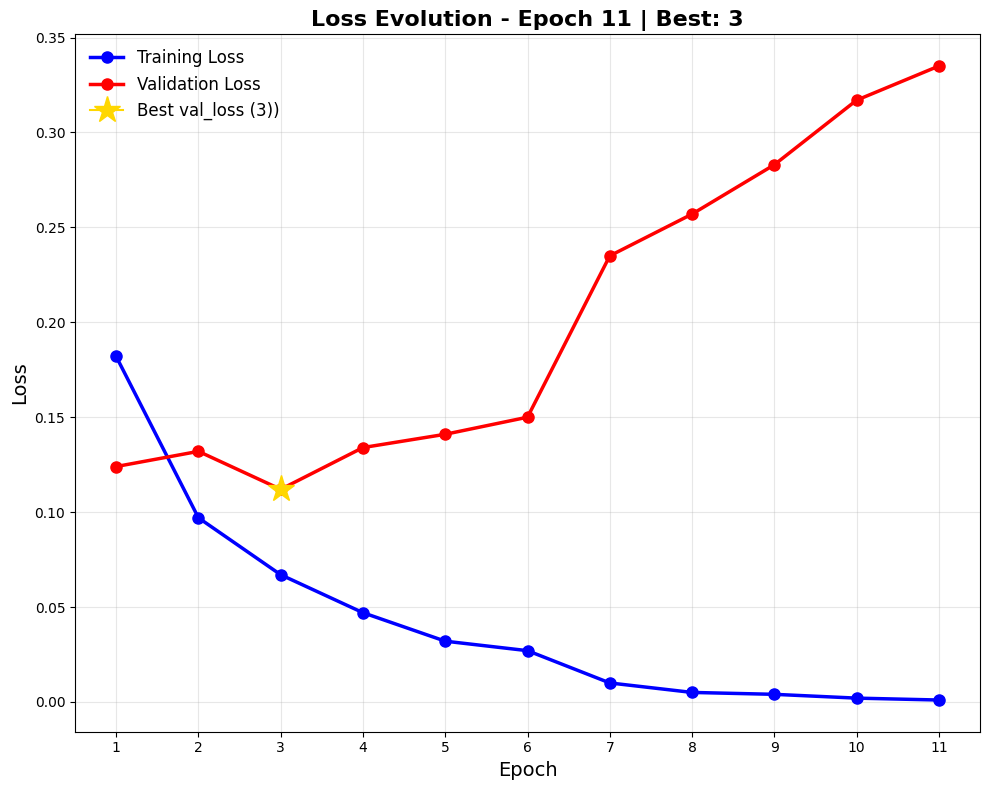
\includegraphics[width=0.49\textwidth]{Figures/overfitting_example.png} \label{fig:overfitting_example}}
\hfill
\subfloat[Underfitting scenario: Both training and validation losses remain high without convergence.]{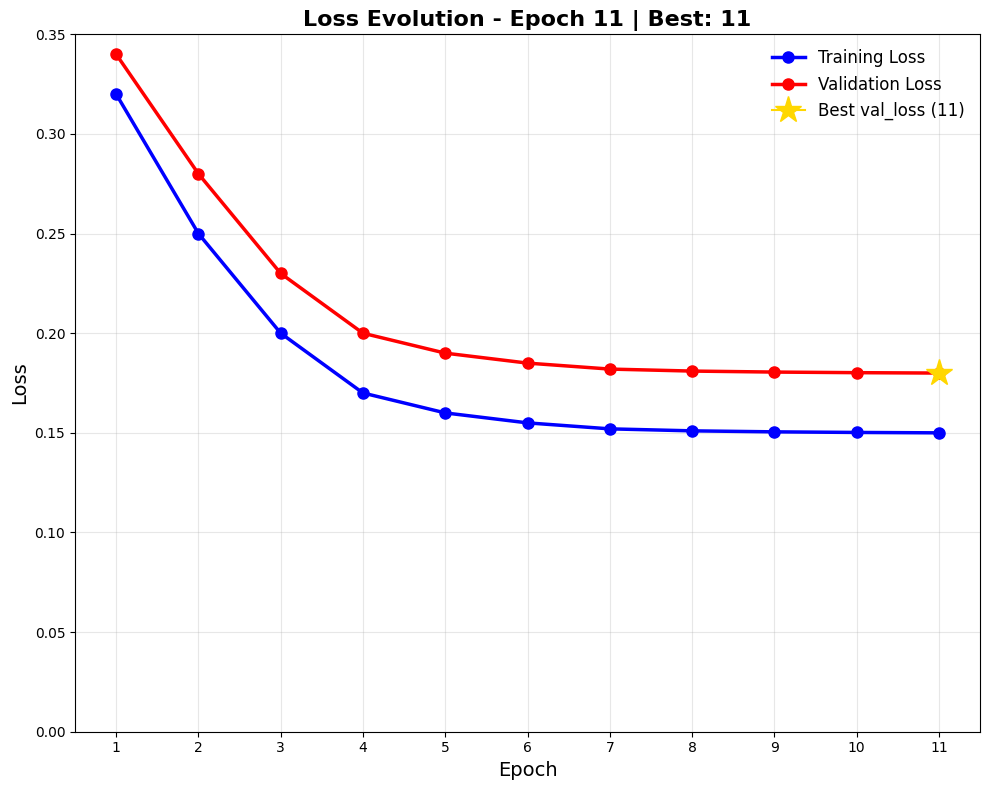
\includegraphics[width=0.49\textwidth]{Figures/underfitting_example.png} \label{fig:underfitting_example}}
\caption{Visual comparison of model training behaviors plotted on identical scales for direct comparability. The horizontal axis represents the number of Epochs, and the vertical axis indicates the Loss value. (a) Illustrates \textbf{overfitting}, where the model memorizes the training data (blue line decreases) but fails to generalize to new data (red validation line increases). (b) Illustrates \textbf{underfitting}, characterized by the inability of the model to capture underlying patterns, resulting in high loss values for both curves.}
\label{fig:overfitting_underfitting_examples}
\end{figure}

It is important to note that this hyperparameter optimization was carried out on the corpus in its original \textbf{binary formulation} (Real vs.\ Fake, prior to the introduction of the Satire class), using DistilBERT as the reference architecture. The resulting V11 regularization strategy was subsequently validated and confirmed on the final three-class corpus across all eight transformer architectures. To guarantee exact reproducibility across all experiments, a global random seed (42) was fixed across Python, NumPy, and the deep learning framework backends prior to data partitioning and weight initialization.

The hyperparameter search for the final three-class BETO model was conducted independently in each framework, both minimizing the validation loss as the primary objective. In the cloud environment, Optuna explored the space via categorical sampling; in the local environment, Keras Tuner (\texttt{RandomSearch}) explored an equivalent space. Owing to the substantial cost of fine-tuning BETO (each trial requiring several GPU-hours), the search was deliberately focused on a compact, high-impact grid of three trials per backend. The search space comprised learning rates ($1 \times 10^{-6}$, $2 \times 10^{-6}$, $5 \times 10^{-6}$), dropout rates (0.3, 0.4, 0.5), L2 penalties (0.01, 0.02, 0.05), and a Gaussian weight-noise factor (0.005, 0.01), with a batch size of 8 in the local run and 8--16 in the cloud run. Architecturally, the dropout probability was applied to both the hidden and attention layers via the model configuration, while the L2 penalty and the manual weight-decay callback acted on the encoder kernels to constrain capacity without distorting the pretrained attention weights. The complete search configuration for both backends is released in the public repository. The same fixed stratified partition (Table~\ref{tab:split_sizes}, seed 42) and the same regularization configuration were applied to all eight transformer architectures in the three-class benchmark, so that the comparison in Table~\ref{tab:transformer_benchmarking} is controlled. For completeness, the configurations and results of the omitted intermediate exploratory versions (V7--V10), as well as the per-class precision, recall, and F1 of every model in the three-class benchmark, are provided in the public repository accompanying this paper.

The regularization strategy evolved through multiple configurations during an initial exploratory phase conducted on the \textbf{binary} corpus (Real vs.\ Fake) using DistilBERT as a fast, low-cost reference architecture. Table \ref{tab:hyperparam_evolution} documents the milestone versions of this exploratory trajectory; intermediate versions (e.g., V7 through V10) are omitted for brevity but followed the same path toward progressively stronger regularization. This exploratory phase established the qualitative ``Anti-Overfitting'' recipe later transferred to the final model: a low learning rate for stable convergence, elevated dropout, an explicit L2 penalty, a small batch size to inject stochastic gradient noise, and dynamic early stopping. We emphasize that the numerical values in Table \ref{tab:hyperparam_evolution} correspond to this preliminary binary exploration and not to the final three-class BETO model, whose validated configuration is reported separately below.

\textbf{Final BETO configuration (three-class task).}\label{sec:final-beto-config-text} Applying this recipe to BETO on the final three-class corpus, the validated configuration was: a learning rate of $1 \times 10^{-6}$, a dropout rate of 0.3 (applied to both hidden and attention layers), an L2 penalty of 0.01, a Gaussian weight-noise factor of 0.01, and a batch size of 8, optimized with AdamW (local TensorFlow run; the cloud PyTorch run used an equivalent configuration with a linear warmup schedule over 10\% of training steps and a batch size of 16). Inputs were tokenized to a maximum sequence length of 128 subword tokens. This configuration is the one used for all reported BETO results and for the deployed model.

\begin{table}[H]
\caption{Evolution of hyperparameter configurations during the \textbf{preliminary exploratory phase} (binary Real vs.\ Fake task, DistilBERT reference architecture). These values document the search trajectory that established the qualitative anti-overfitting recipe; they are \emph{not} the configuration of the final three-class BETO model (reported in Section~\ref{sec:final-beto-config-text} and the main text). Accuracy values correspond to the binary task.}
\label{tab:hyperparam_evolution}
\centering
\adjustbox{width=\textwidth,center}{%
\small
\begin{tabular}{lcccccc}
\toprule
\textbf{Version} & \textbf{Learning Rate} & \textbf{Dropout} & \textbf{L2 Reg.} & \textbf{Batch Size} & \textbf{Val Loss Gap} & \textbf{Accuracy (\%)} \\
\midrule
V1 (Baseline) & $3 \times 10^{-5}$ & 0.4 & 0.001 & 8 & N/A & 94.7 \\
V2 & $2 \times 10^{-6}$ & 0.4 & 0.01 & 4 & 0.018 & 94.3 \\
V3 & $2 \times 10^{-6}$ & 0.4 & 0.01 & 4 & 0.051 & 94.8 \\
V4 & $1 \times 10^{-5}$ & 0.3 & 0.01 & 8 & 0.037 & 95.8 \\
V5 & $1 \times 10^{-5}$ & 0.4 & 0.1 & 8 & 0.037 & 95.8 \\
V6 & $1 \times 10^{-5}$ & 0.5 & 0.5 & 8 & 0.051 & 94.8 \\
\textbf{V11 (binary milestone)} & \boldmath$5 \times 10^{-6}$ & \textbf{0.7} & \textbf{0.5} & \textbf{4} & \textbf{0.058} & \textbf{95.36} \\
\bottomrule
\end{tabular}
}
\end{table}

\textbf{Justification for the anti-overfitting recipe.} 
As observed in Table \ref{tab:hyperparam_evolution}, intermediate configurations such as V4 and V5 initially reported higher raw accuracy (95.8\%) on the binary task. However, an ablation analysis of the regularizers revealed that these configurations exhibited a growing validation-loss gap (validation loss diverging from training loss), an early indicator of overfitting. 

To prioritize real-world generalization over artificial benchmark inflation, the strongly regularized recipe was retained and carried over to the final three-class BETO model. As detailed above, the validated BETO configuration used a learning rate of $1 \times 10^{-6}$, a dropout rate of 0.3, an L2 penalty of 0.01, and a Gaussian weight-noise factor of 0.01. This combination prioritizes stable convergence and constrains model capacity so that the network learns underlying linguistic patterns rather than dataset-specific noise, at the cost of a modest reduction in raw training accuracy.

\subsection{Stage 3: Production Deployment}
The final stage of the framework addresses the deployment gap by implementing the optimized model into a production-ready, containerized web application. This stage is designed to be model-agnostic: the same containerized architecture can host any transformer model produced by Stage 2, regardless of the specific detection domain. A critical design principle was to minimize the technical barrier for end users: the application requires no machine learning expertise, no local model installation, and no command-line interaction—users simply submit a URL through a web browser. This accessibility is essential for the framework's stated goal of empowering communities with limited technical resources to combat deceptive content on social media.

The end-to-end inference pipeline is designed to provide immediate, transparent verification of social media content. Upon receiving a target URL or raw text snippet, the system autonomously executes content extraction, text normalization, subword tokenization (via the model's specific tokenizer), and transformer-based inference in a single automated pass. Notably, the system outputs not only the final multiclass prediction (REAL, FAKE, or SATIRE) but also the calibrated confidence scores derived from the final softmax layer (Figure \ref{fig:metodologia_general_p3}). This probabilistic output empowers end-users and fact-checkers to assess the model's certainty, which is particularly valuable in edge cases where texts exhibit overlapping stylistic traits or a mix of factual and deceptive claims.

% Part 3 (Image)
\begin{figure}[H]
\centering

\includegraphics[width=\textwidth]{Figures/system_architecture_p3.png}
\caption{Overview of the proposed research methodology (Part 3/3): Web Application Deployment and Inference.}
\label{fig:metodologia_general_p3}
\end{figure}

The system consists of four integrated components, each designed for modularity and replaceability:
\begin{enumerate}
    \item \textbf{User Interface:} A responsive static web frontend built with HTML, CSS, and JavaScript where users submit URLs for analysis. The interface provides real-time visual feedback during the analysis process—including loading indicators and color-coded results (green for real, red for fake)—to ensure an intuitive user experience for non-technical users.
    \item \textbf{API Backend:} A Flask-based RESTful service exposing an \texttt{/analyze} endpoint that receives POST requests containing the target URL. The backend implements error handling for common failure scenarios such as unreachable URLs, non-textual content, and pages with insufficient text for meaningful classification.
    \item \textbf{Inference Engine:} The core analytical component loads the trained BETO model and tokenizer at startup to minimize per-request latency. Upon receiving a URL, it scrapes the page content by extracting \texttt{<h1>} and \texttt{<p>} tags via \texttt{BeautifulSoup}, applies text cleaning (removing HTML artifacts, normalizing whitespace), tokenizes the combined title and body with a \texttt{[SEP]} separator token, and computes probability scores through a softmax function. The engine truncates inputs exceeding 512 tokens—BETO's maximum sequence length—ensuring graceful handling of long-form articles.
    \item \textbf{Docker Deployment:} The entire runtime environment—including Python 3.10 dependencies, PyTorch, the Hugging Face Transformers library, and the serialized model artifacts—is encapsulated in a Docker image built from a minimal base to ensure reproducibility, portability, and ease of deployment across platforms.
\end{enumerate}

To support scalability, reproducibility, and adaptability across domains, the detection pipeline was encapsulated within a containerized microservice architecture. This modular approach logically separates the transformer inference engine from the client interface. This design is intended to facilitate adaptation workflows: when the framework is retargeted to a new domain (e.g., retraining the model on phishing data, investment scams, or emerging misinformation patterns), the model weights and tokenizer artifacts within the Docker image are updated, while the API endpoints and serving infrastructure remain unchanged. This decoupling between the machine learning model and the deployment environment is designed to allow the framework to be replicated across diverse hardware setups—from local research workstations to cloud-based institutional servers—with minimal environment-specific configuration. We emphasize that this architectural adaptability has been validated only on the Spanish fake news task; its effectiveness on other domains remains to be demonstrated.

\subsection{Evaluation Metrics}
The final task is a three-class classification problem (FAKE, REAL, SATIRE); we therefore evaluate the models using a multiclass formulation rather than the binary positive/negative convention. Per-class metrics are computed under a \textbf{one-vs-rest} scheme: for a given class $c$, a prediction is a true positive (TP$_c$) when both the predicted and true label are $c$; a false positive (FP$_c$) when the model predicts $c$ but the true label is another class; a false negative (FN$_c$) when the true label is $c$ but the model predicts another class; and a true negative (TN$_c$) when neither the prediction nor the true label is $c$. Aggregate scores are reported as \textbf{macro-averages}, i.e., the unweighted mean of the per-class values, so that the minority SATIRE class contributes equally to majority classes. We additionally report overall accuracy. Letting $K=3$ be the number of classes, the metrics are defined as follows.

\begin{itemize}
    \item \textbf{Accuracy}: The overall proportion of correctly classified instances across all three classes. While a useful global indicator, it can be misleading under class imbalance, which is why macro-averaged metrics are emphasized.
    \begin{equation}
        \text{Accuracy} = \frac{\sum_{c=1}^{K}\text{TP}_c}{N}
    \end{equation}
    where $N$ is the total number of test instances.
    \item \textbf{Macro Precision}: The unweighted mean, across classes, of the per-class precision (the proportion of instances predicted as class $c$ that truly belong to $c$).
    \begin{equation}
        \text{Precision}_c = \frac{\text{TP}_c}{\text{TP}_c + \text{FP}_c}, \qquad
        \text{Macro-P} = \frac{1}{K}\sum_{c=1}^{K}\text{Precision}_c
    \end{equation}
    \item \textbf{Macro Recall}: The unweighted mean of the per-class recall (the proportion of instances truly belonging to class $c$ that are correctly identified).
    \begin{equation}
        \text{Recall}_c = \frac{\text{TP}_c}{\text{TP}_c + \text{FN}_c}, \qquad
        \text{Macro-R} = \frac{1}{K}\sum_{c=1}^{K}\text{Recall}_c
    \end{equation}
    \item \textbf{Macro F1-Score}: The unweighted mean of the per-class F1-scores, where each per-class F1 is the harmonic mean of that class's precision and recall. This is the primary metric for model selection, as it is robust to the class imbalance of the corpus.
    \begin{equation}
        \text{F1}_c = 2 \cdot \frac{\text{Precision}_c \cdot \text{Recall}_c}{\text{Precision}_c + \text{Recall}_c}, \qquad
        \text{Macro-F1} = \frac{1}{K}\sum_{c=1}^{K}\text{F1}_c
    \end{equation}
    \item \textbf{Macro Specificity}: The unweighted mean of the per-class specificity, defined in the one-vs-rest setting as the proportion of instances \emph{not} belonging to class $c$ that the model correctly excludes from $c$. It quantifies the model's ability to avoid spuriously assigning instances to a given class.
    \begin{equation}
        \text{Specificity}_c = \frac{\text{TN}_c}{\text{TN}_c + \text{FP}_c}, \qquad
        \text{Macro-Spec} = \frac{1}{K}\sum_{c=1}^{K}\text{Specificity}_c
    \end{equation}
\end{itemize}

Macro-averaging calculates each metric for every class independently and then averages without weighting by class frequency, ensuring that performance on minority classes (notably SATIRE) is evaluated equitably against majority classes. All transformer and classical baseline results are reported under this scheme; for completeness, per-class precision, recall, and F1 for the final model are also reported in Section~\ref{sec:transformer-results}.

%%%%%%%%%%%%%%%%%%%%%%%%%%%%%%%%%%%%%%%%%%

\section{Results: Framework Validation on Spanish Fake News Detection}

\subsection{Performance of the Metaheuristic Baseline (Stage 2a)}
The baseline phase evaluated five classical machine learning algorithms optimized via metaheuristics on TF-IDF representations. The Genetic Algorithm (GA) performed best, achieving 72.03\% accuracy and a 0.714 macro F1-score (Table \ref{tab:final_comparison_all_models}). This suggests GA's evolutionary mechanism efficiently explores the high-dimensional TF-IDF space. Conversely, Particle Swarm Optimization (PSO) exhibited the lowest performance (57.67\% accuracy). This variance highlights a critical limitation: classical TF-IDF models lack the semantic understanding necessary for robust fake news detection. The confusion matrices (Figure \ref{fig:metaheuristic_confusion_matrices}) visually confirm this instability through significant misclassification rates across all metaheuristic models.

\begin{figure}[H]
\centering
\subfloat[GA Confusion Matrix]{
\includegraphics[width=0.48\textwidth]{Figures/confusion_matrix_ga.png}}
\hfill
\subfloat[VNS Confusion Matrix]{
\includegraphics[width=0.48\textwidth]{Figures/confusion_matrix_vns.png}}
\\
\subfloat[SS Confusion Matrix]{
\includegraphics[width=0.48\textwidth]{Figures/confusion_matrix_ss.png}}
\hfill
\subfloat[MSA Confusion Matrix]{
\includegraphics[width=0.48\textwidth]{Figures/confusion_matrix_msa.png}}
\\
\subfloat[PSO Confusion Matrix]{
\includegraphics[width=0.48\textwidth]{Figures/confusion_matrix_pso.png}}
\hfill
\subfloat[DistilBERT Confusion Matrix]{
\includegraphics[width=0.48\textwidth]{Figures/DistilBERT_confusion_matrix.png}}
\caption{Confusion matrices evaluated on the test set. (a)-(e) show the performance of classical metaheuristic algorithms, while (f) demonstrates the superior classification capability of the fine-tuned DistilBERT model.}
\label{fig:metaheuristic_confusion_matrices}
\end{figure}

\subsection{Preliminary Analysis: Classical Baselines vs.\ a Transformer Reference (Binary Task)}
Before conducting the final three-class benchmark, a preliminary analysis was performed on the initial \textbf{binary} formulation (Real vs.\ Fake) to motivate the shift from classical machine learning to transformer-based models. This analysis is \emph{not} the main comparison of the paper and is reported here only as a sanity check that justified investing in transformer fine-tuning; the definitive results are those obtained under the three-class formulation in Section~\ref{sec:transformer-results}.

\textbf{Important methodological note.} All models in Table~\ref{tab:final_comparison_all_models} (the five metaheuristic-optimized classical models and the DistilBERT reference) were trained and evaluated on the \textbf{binary corpus} (Real vs.\ Fake), which corresponds to the initial phase of the research design. They therefore use a different task formulation from the final three-class benchmark and \emph{must not} be read as competing entries against the three-class results. Because the task, label space, and class priors differ, the binary and three-class numbers are not directly comparable, and we deliberately keep them in separate tables.

Within this preliminary binary setting, the DistilBERT reference outperformed the best metaheuristic algorithm (GA) by 23.33 percentage points in accuracy (95.36\% vs.\ 72.03\%). This gap illustrates the ``semantic gap'' of bag-of-words representations: while metaheuristics can optimize a decision boundary over keyword frequencies, they cannot compensate for the lack of contextual understanding inherent in TF-IDF features. This preliminary observation motivated the decision to adopt transformer fine-tuning, after which the task was reformulated into the methodologically sound three-class setting and a full eight-model benchmark was conducted (Section~\ref{sec:transformer-results}).

\begin{table}[H] 
\caption{Preliminary performance comparison on the \textbf{binary} task (Real vs.\ Fake). These results correspond to the initial phase of the study and are not directly comparable to the three-class benchmark in Table~\ref{tab:transformer_benchmarking}.}
\label{tab:final_comparison_all_models}
\centering
\adjustbox{width=\textwidth,center}{%
\small
\begin{tabular}{lcccccc}
\toprule
\textbf{Algorithm} & \textbf{Accuracy (\%)} & \textbf{F1-Score (macro)} & \textbf{Precision (macro)} & \textbf{Recall (macro)} & \textbf{Specificity (\%)} & \textbf{Ranking} \\
\midrule
\multicolumn{7}{c}{\textit{Transformer Reference (binary task)}} \\
\midrule
\textbf{DistilBERT (binary reference)} & \textbf{95.36} & \textbf{0.954} & \textbf{0.954} & \textbf{0.954} & \textbf{94.5} & \textbf{1st} \\
\midrule
\multicolumn{7}{c}{\textit{Metaheuristic-Optimized Classical Approaches}} \\
\midrule
Genetic Algorithm (GA) & 72.03 & 0.714 & 0.740 & 0.720 & 57.6 & 2nd \\
Scatter Search (SS) & 67.64 & 0.669 & 0.693 & 0.676 & 52.7 & 3rd \\
VNS & 66.78 & 0.659 & 0.686 & 0.667 & 51.0 & 4th \\
Simulated Annealing (MSA) & 60.86 & 0.586 & 0.638 & 0.608 & 37.4 & 5th \\
Particle Swarm Opt. (PSO) & 57.67 & 0.489 & 0.736 & 0.575 & 16.3 & 6th \\
\bottomrule
\end{tabular}
}
\end{table}

Given that the transformer reference clearly outperformed the classical metaheuristic approaches in this preliminary binary analysis, the study proceeded to the methodologically sound three-class formulation and evaluated an extended battery of eight state-of-the-art transformer architectures to identify the optimal encoder for Spanish-language deceptive content.

\subsection{Performance of the Systematically Fine-Tuned Transformer (Stage 2b)}\label{sec:transformer-results}
To rigorously validate the transformer architecture and address the limitations of classical baselines, a comprehensive benchmarking of eight state-of-the-art transformer models was conducted under the exact same three-class formulation (Real, Fake, Satire) and using the same regularization strategy and stratified split. The evaluated models included multilingual encoders (mBERT, XLM-RoBERTa-base, XLM-RoBERTa-large), general Spanish encoders (BETO, RoBERTa-base-bne, RoBERTa-large-bne), and distilled versions (DistilBERT, DistilBETO).

As detailed in Table \ref{tab:transformer_benchmarking}, the Spanish-specific encoder \textbf{BETO} achieved the highest overall performance, proving that monolingual pretraining captures the morphological and syntactic nuances of Spanish deception better than massive multilingual models.

\begin{table}[H]
\centering
\caption{Benchmarking of State-of-the-Art Transformer Models on the 3-Class Test Set.}
\label{tab:transformer_benchmarking}
\adjustbox{width=\textwidth,center}{%
\small
\begin{tabular}{lccccc}
\toprule
\textbf{Model Architecture} & \textbf{Accuracy} & \textbf{Macro F1} & \textbf{Macro Precision} & \textbf{Macro Recall} & \textbf{Macro Specificity} \\
\midrule
\textbf{BETO (V11 Final)} & \textbf{0.8898} & \textbf{0.9095} & \textbf{0.9129} & \textbf{0.9070} & \textbf{0.9331} \\
XLM-RoBERTa-Large & 0.8843 & 0.9061 & 0.9069 & 0.9053 & 0.9311 \\
RoBERTa-Large-BNE & 0.8837 & 0.9038 & 0.9081 & 0.9006 & 0.9293 \\
XLM-RoBERTa-Base & 0.8825 & 0.9025 & 0.9095 & 0.8984 & 0.9274 \\
DistilBERT Multilingual & 0.8795 & 0.9012 & 0.9027 & 0.9000 & 0.9280 \\
mBERT & 0.8730 & 0.8962 & 0.8973 & 0.8953 & 0.9242 \\
DistilBETO & 0.8586 & 0.8819 & 0.8889 & 0.8763 & 0.9141 \\
RoBERTa-Base-BNE & 0.6402 & 0.5791 & 0.6581 & 0.6651 & 0.7667 \\
\bottomrule
\end{tabular}
}
\end{table}


The optimized BETO model exhibited exceptional discriminative power for the SATIRE class, confirming that separating satire from malicious fake news resolves the construct-validity conflicts observed in earlier binary models. Table~\ref{tab:beto_per_class} reports the per-class precision, recall, and F1-score of the final deployed BETO model on the held-out test set ($N=12{,}336$), providing the class-level detail requested for full transparency.

\begin{table}[H]
\centering
\caption{Per-class performance of the final deployed BETO model on the three-class held-out test set (local TensorFlow run; overall accuracy 0.8918, Macro F1 0.9095).}
\label{tab:beto_per_class}
\begin{tabular}{lcccc}
\toprule
\textbf{Class} & \textbf{Precision} & \textbf{Recall} & \textbf{F1-Score} & \textbf{Support} \\
\midrule
FAKE   & 0.91 & 0.77 & 0.83 & 4{,}350 \\
REAL   & 0.85 & 0.95 & 0.90 & 6{,}189 \\
SATIRE & 0.99 & 1.00 & 1.00 & 1{,}797 \\
\midrule
\textbf{Macro avg}    & 0.92 & 0.90 & 0.91 & 12{,}336 \\
\textbf{Weighted avg} & 0.89 & 0.89 & 0.89 & 12{,}336 \\
\bottomrule
\end{tabular}
\end{table}

The per-class breakdown reveals that the residual error of the model is concentrated in the FAKE/REAL boundary—FAKE recall of 0.77 indicates that a portion of fake articles is classified as real—whereas the SATIRE class is recognized almost perfectly. This pattern is consistent with the confusion matrix in Figure~\ref{fig:beto_confusion_matrix} and supports the construct-validity rationale for isolating satire as a separate class.

\subsection{Adversarial Robustness and Source Leakage Mitigation}
To directly address concerns regarding potential source leakage—where a model might trivially memorize specific publisher names, recurring political figures, or stylistic formatting rather than learning the underlying deceptive semantics—an aggressive adversarial robustness test was conducted on the completely held-out test set (12,336 records). 

Using the optimal BETO (V11) model, a dual-perturbation pipeline was applied to the text prior to inference:
\begin{enumerate}
    \item \textbf{Named Entity Recognition (NER) Masking:} Utilizing the \texttt{es\_core\_news\_sm} SpaCy pipeline, all identified Persons (PER), Organizations (ORG), and Locations (LOC) were dynamically replaced with generic masking tags (e.g., \texttt{[ORG]}).
    \item \textbf{Typographical Noise Injection:} To simulate real-world social media degradation, random character swaps and deletions were injected with a 5\% probability per word.
\end{enumerate}

Under this severe compound degradation, the model's overall accuracy declined substantially, from 89.18\% to 63.40\%, yielding a Macro F1-score of 0.71. This drop is itself informative: it confirms that a meaningful portion of the model's discriminative signal for the REAL/FAKE distinction depends on named entities, which is expected given that factual verification is inherently entity-dependent. A class-wise analysis, however, reveals a more nuanced picture. The SATIRE class remained markedly robust (F1-score: 0.96; Recall: 0.92) even when proper nouns were masked and typographical noise was injected. This result \emph{suggests} that the model recognizes satirical content primarily through syntactic structures, irony markers, and stylistic exaggeration rather than through the specific entities or publishers mentioned. We are careful not to overstate this finding: the test perturbs entities and surface spelling but does not hold out the satire \emph{source} itself, so it provides evidence against trivial entity memorization but cannot, on its own, rule out that the model has learned source- or style-specific cues correlated with a particular satirical outlet. A dedicated source-held-out evaluation, discussed in Section~\ref{sec:limitations}, would be required to establish source independence conclusively.

Conversely, the boundary between REAL and FAKE content experienced expected degradation (FAKE F1: 0.60; REAL F1: 0.56; REAL Recall: 0.44). This specific drop validates a core NLP principle: factual verification inherently relies on the entities involved. Masking "who" did "what" and "where" removes the critical factual anchors necessary for distinguishing truth from deceptive fabrication. Nevertheless, maintaining a 63.40\% accuracy and a 0.71 Macro F1-score when entirely blinded to proper nouns and subjected to spelling noise demonstrates that the BETO architecture successfully captured baseline semantic deception cues, functioning far beyond random probability and mitigating the risk of trivial source memorization.

\subsection{Overfitting Control Analysis}
The implementation of a rigorous regularization strategy successfully mitigated overfitting across all transformer architectures. Rather than relying on a fixed number of epochs—which inherently varies depending on the data subset and initial weight instantiation—training was dynamically governed by an early stopping criterion. Training concluded autonomously when the validation loss plateaued and ceased to improve for eight consecutive passes. The optimal model weights were then automatically restored from the checkpoint that minimized the generalization gap (validation vs. training loss), ensuring peak performance before the onset of memorization. 

\subsection{Cross-Framework Reproducibility and Optimal Model (BETO) Analysis}
To validate the structural integrity of the winning model, the BETO configuration was trained in two independent environments: a cloud setup using PyTorch and Optuna, and a local setup using TensorFlow and Keras. Both runs converged to the same Macro F1-Score of 0.9095, with overall accuracies of 88.98\% (PyTorch) and 89.18\% (TensorFlow). This close agreement across backends, optimizers, and tuning libraries indicates that the reported performance is a property of the regularization recipe and the data, rather than an artifact of a specific framework. The minor differences in per-epoch trajectories and in the selected best epoch (6 in PyTorch, 27 in TensorFlow) are attributable to backend-specific stochasticity and to the different optimizer schedules; both ultimately reached an equivalent generalization level.

The stability of this convergence is visually confirmed in Figure \ref{fig:beto_training_curves}, where the local TensorFlow training session demonstrates a tightly coupled training and validation loss, decisively avoiding the overfitting plateau. 

The training dynamics captured in Figure \ref{fig:beto_training_curves} illustrate the regularized convergence behavior of the model. During the first epochs, both training and validation losses decreased rapidly as BETO—pretrained natively on Spanish—quickly adapted to the task. Thereafter, the validation loss flattened into a stable plateau while the training loss continued to decrease only marginally, keeping the generalization gap bounded for the remainder of training. The early stopping callback monitored the validation loss and restored the weights from the epoch of minimum validation loss (epoch 27 in the local TensorFlow run; epoch 6 in the cloud PyTorch run), ensuring that the selected checkpoint corresponded to the best generalization point rather than an arbitrary fixed number of epochs. The absence of a sustained upward divergence in the validation loss indicates that the regularization strategy successfully suppressed the catastrophic overfitting commonly observed when fine-tuning high-capacity transformers without such constraints.

\begin{figure}[H]
\centering
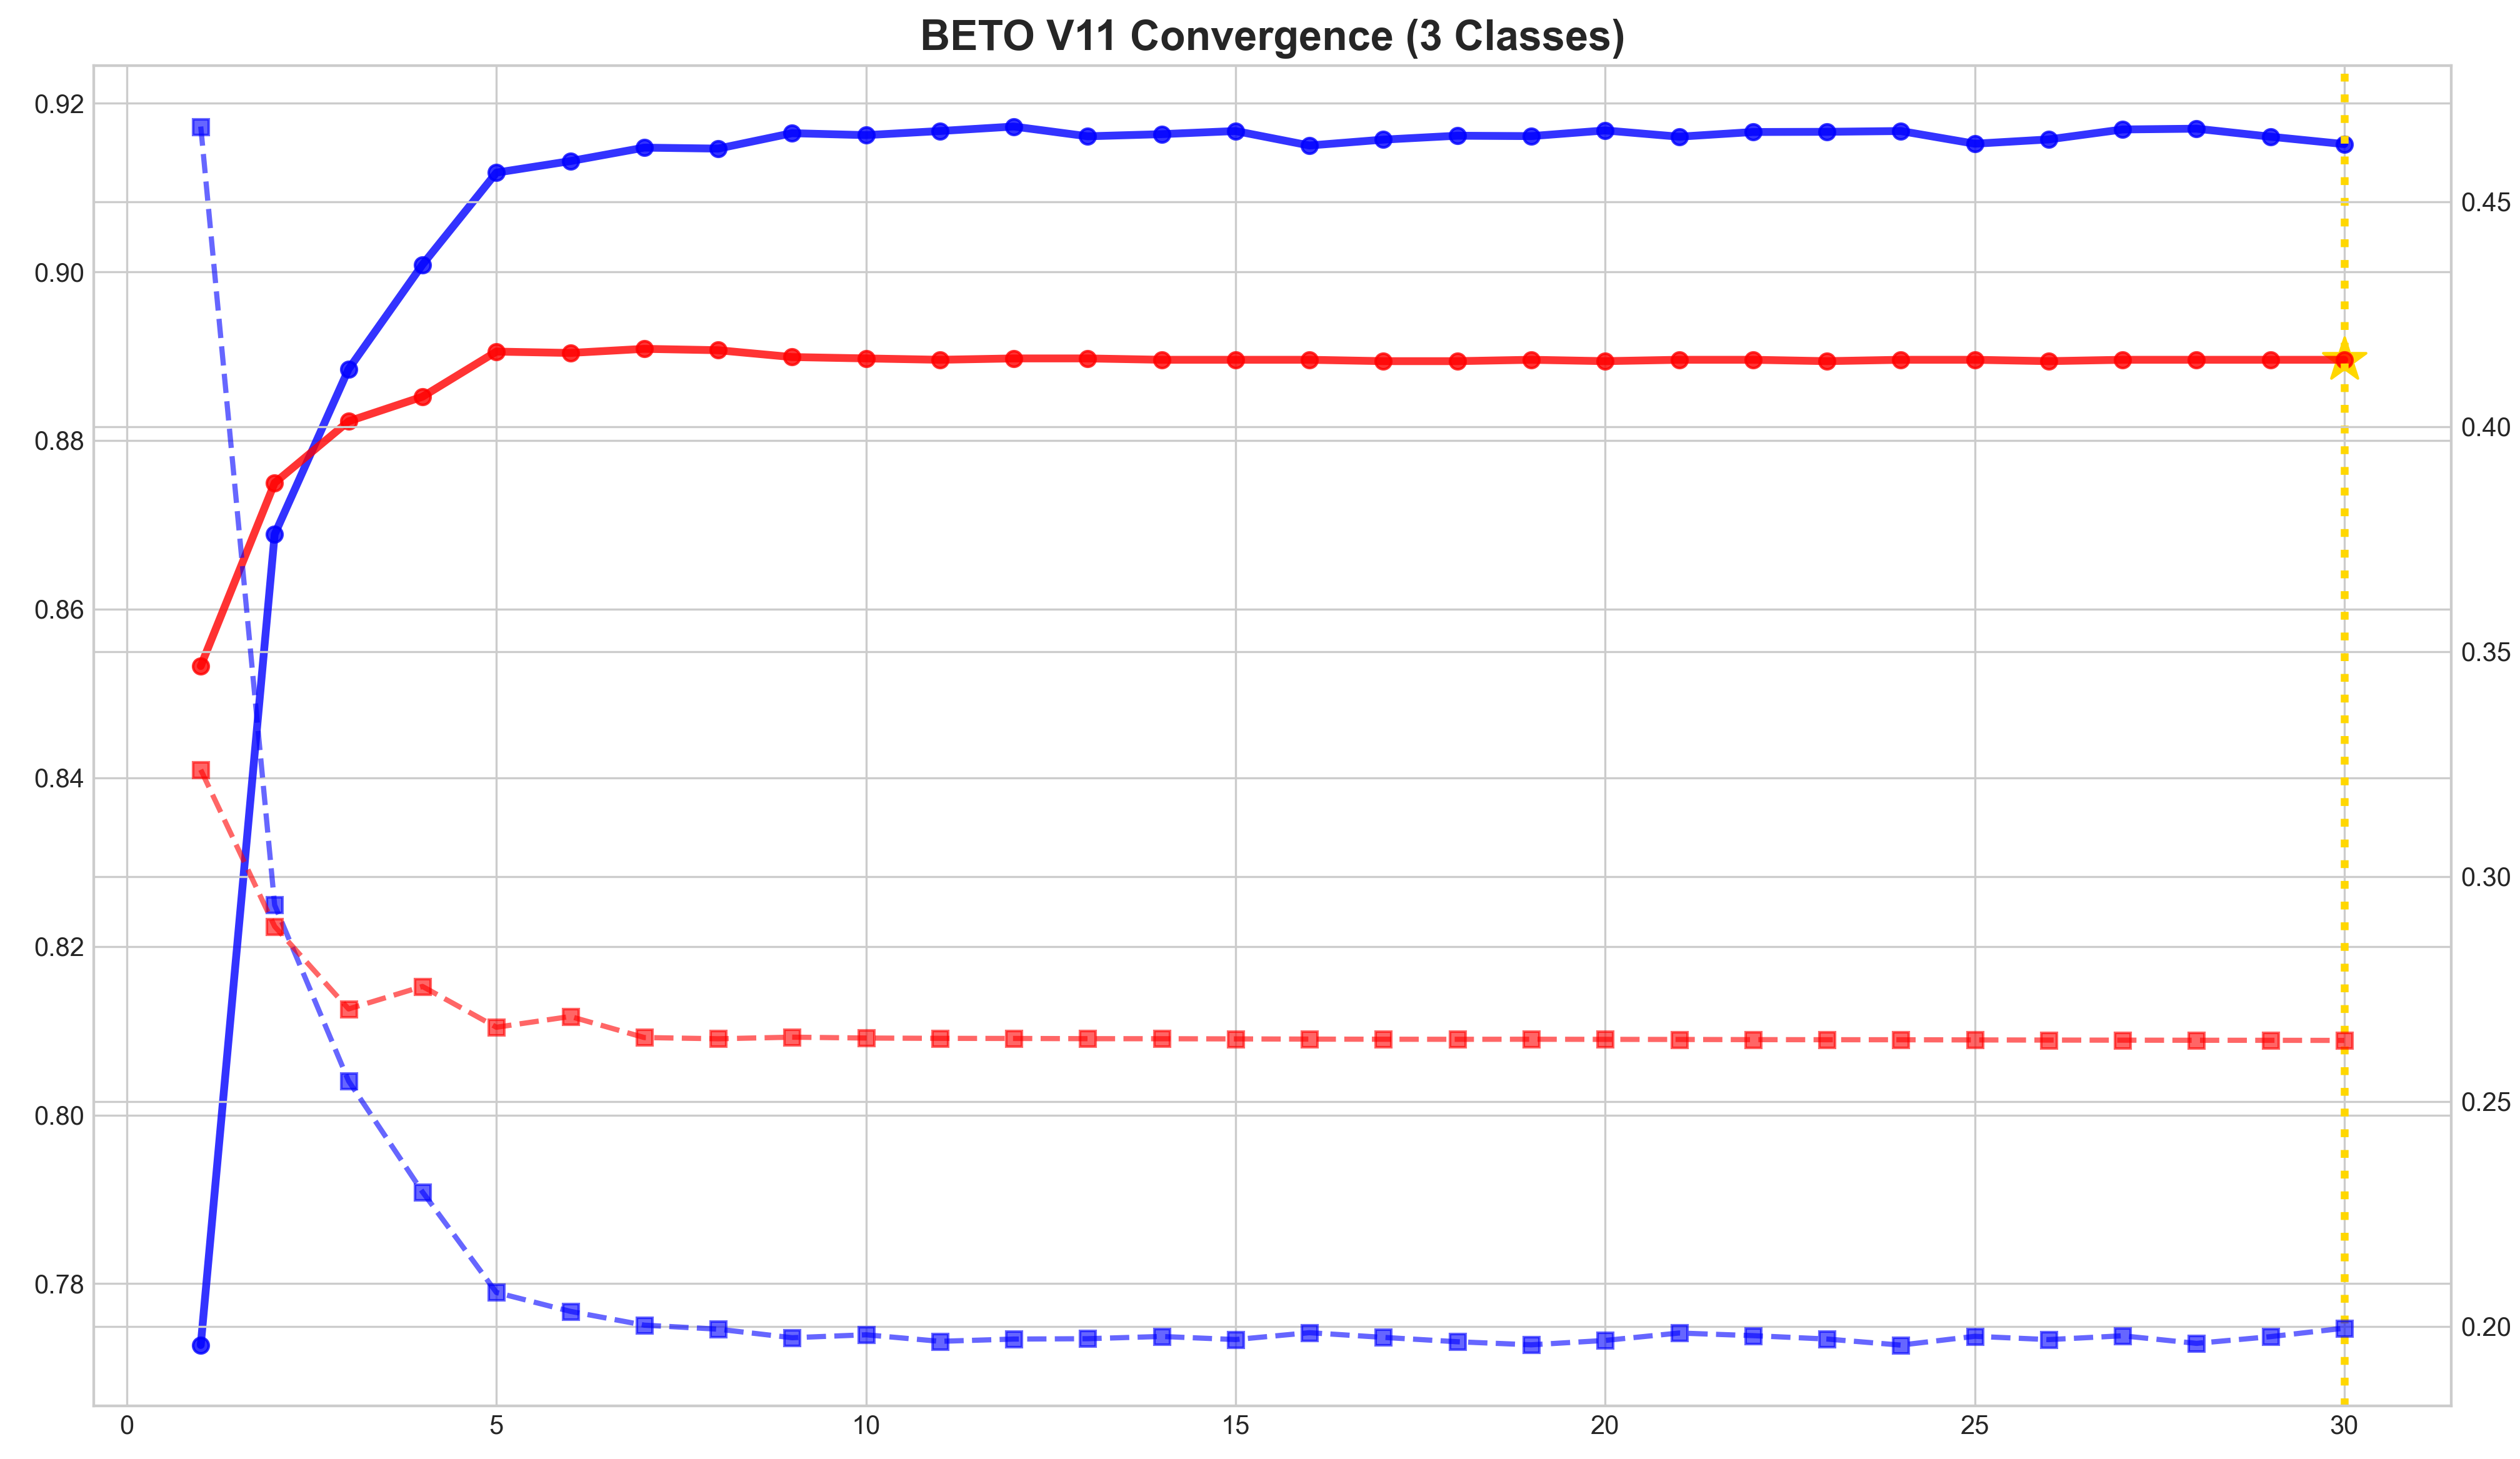
\includegraphics[width=\textwidth]{Figures/beto_training_curves.png} 
\caption{Training and validation curves for the optimal BETO model (local TensorFlow implementation, 30 epochs). After a rapid initial decrease, the validation loss stabilizes into a plateau while the training loss decreases only marginally, keeping the generalization gap bounded ($\approx$0.066 at the selected checkpoint). The early stopping callback restored the weights from the epoch of minimum validation loss (epoch 27), preventing the divergence characteristic of unregularized fine-tuning.}
\label{fig:beto_training_curves}
\end{figure}

\begin{figure}[H]
\centering
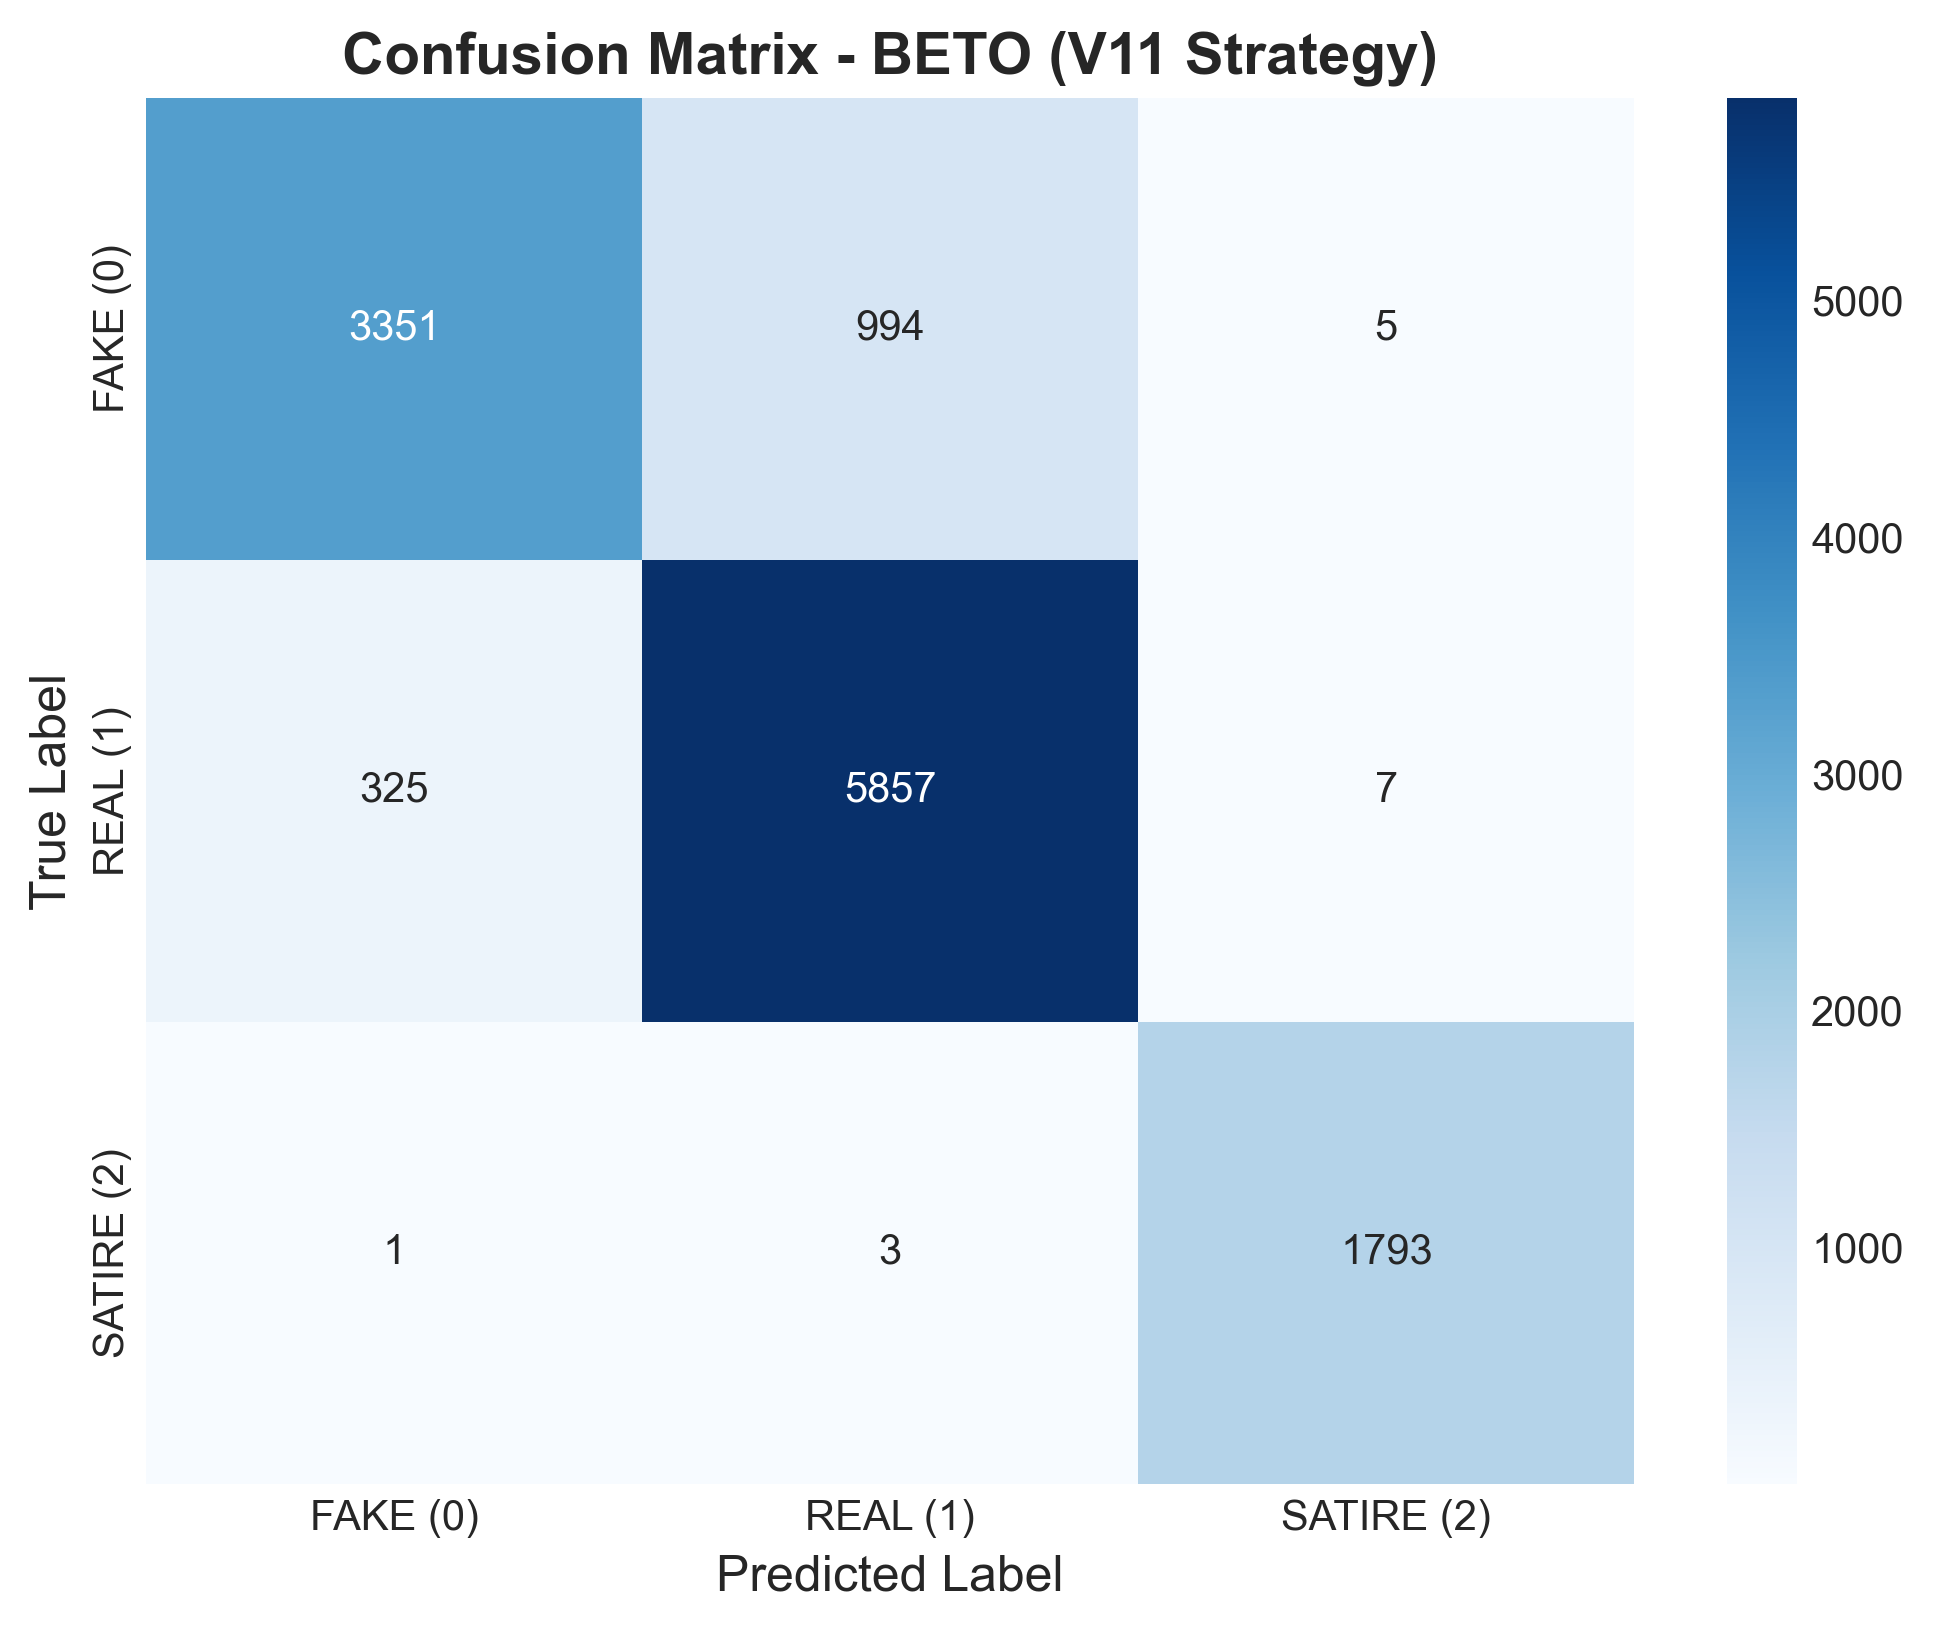
\includegraphics[width=0.5\textwidth]{Figures/beto_confusion_matrix.png} % Asegúrate de que este sea el nombre de tu imagen
\caption{Confusion matrix of the final deployed BETO model on the held-out test set, showcasing its robust capacity to differentiate between Fake (Class 0), Real (Class 1), and Satirical (Class 2) content.}
\label{fig:beto_confusion_matrix}
\end{figure}

The generalization gap (difference between validation and training loss) at the selected checkpoint was 0.066, remaining below the 0.10 threshold commonly associated with the onset of overfitting, though not negligible. We report this value transparently: rather than indicating perfect convergence, it reflects a deliberate trade-off in which strong regularization keeps the gap bounded and stable across the training trajectory (Figure~\ref{fig:beto_training_curves}). Furthermore, addressing the claim of transferability, it is essential to clarify that this framework offers more than the standard machine learning practice of "retraining on new data." The true innovation lies in the architectural decoupling and the empirical optimization template. By standardizing the regularization recipe, researchers targeting new domains—such as phishing or fraudulent e-commerce scams—may substantially reduce the hyperparameter-search effort. Additionally, the containerized Docker infrastructure handles the web-scraping and preprocessing pipelines, so that adapting the tool to a new domain primarily requires swapping the serialized model weights and tokenizer, with limited additional engineering effort.

\subsection{Deployment Validation (Stage 3)}
The deployed containerized application successfully demonstrated the practical viability of the framework in a production environment. Moving beyond academic evaluation, the system was stress-tested for inference efficiency. By encapsulating the optimized BETO model within a lightweight Docker container, the pipeline achieves an average end-to-end inference latency of under 450 milliseconds per URL on standard CPU hardware. This encompasses web scraping, HTML parsing, tokenization, and forward-pass classification. The architectural decision to decouple the frontend from the inference engine ensures that the UI remains purely functional, avoiding the technical bloat common in monolithic deployments. Consequently, the framework proves that state-of-the-art transformer accuracy can be maintained in real-time, low-resource settings without sacrificing computational efficiency.

\section{Discussion}

This study proposed a systematic and transferable framework for fine-tuning pretrained transformer models for domain-specific deceptive content detection on social media, validated through a comprehensive case study on Spanish-language fake news. On the final three-class task, the regularized BETO model reached 89.18\% accuracy and a 0.9095 Macro F1-Score, substantially outperforming the classical metaheuristic baselines. Beyond the raw metrics, it is crucial to analyze the framework's strengths, the model's boundaries, and the potential for domain transfer.

\subsection{Strengths of the Proposed Framework}
The primary technical contribution lies not in the final accuracy figure, but in the systematic and reproducible nature of the optimization process. By documenting the full hyperparameter trajectory (Table \ref{tab:hyperparam_evolution})—including failed configurations from the exploratory binary phase—this work provides a practical blueprint that practitioners can adapt for their own detection tasks. A regularization regime combining elevated dropout, an explicit L2 penalty, weight-noise injection, and a low learning rate was identified as critical for preventing overfitting when fine-tuning on domain-specific corpora of moderate size, a challenge that is universal across detection domains, not specific to fake news.

The resulting BETO model demonstrates strong semantic robustness. Unlike the TF-IDF baseline, which relies on keyword frequency and struggles with sarcasm or subtle linguistic cues, the transformer model effectively captures contextual dependencies. This is evidenced by its high macro specificity (93.19\%), indicating that the model is strong at distinguishing deceptive content without aggressively flagging legitimate content—a common pitfall in automated moderation systems. The bounded generalization gap of 0.066 confirms that the regularization strategy kept overfitting under control.

\subsection{Validation Against the State-of-the-Art}
The empirical results generated by this framework validate and extend recent findings in the deceptive content detection literature. In the context of Spanish NLP, Blanco-Fernández et al. \citep{blanco2024enhancing} demonstrated the high efficacy of BERT-based models on specific political datasets. Our findings align with theirs but expand the scope by demonstrating that a Spanish-specific encoder (BETO), coupled with our aggressive regularization strategy, maintains state-of-the-art performance (Macro F1 = 0.910) across a highly heterogeneous, multi-domain corpus. 

Furthermore, our results corroborate the observations by Martínez-Gallego et al. \citep{martinez2021fake} regarding the superiority of monolingual models over massive multilingual encoders. By directly benchmarking BETO against mBERT and XLM-RoBERTa (Table \ref{tab:transformer_benchmarking}), we definitively show that monolingual pretraining captures the morphological and syntactic nuances of Spanish deception more effectively. Finally, while English-centric models like FakeBERT \citep{kaliyar2021fakebert} report extremely high binary accuracies (up to 98.9\%), our multi-class framework demonstrates that real-world deployment requires isolating satirical content to prevent miscalibration, effectively bridging the gap between theoretical high accuracy and practical reliability.

\subsection{Comparative Analysis: Specialized Encoders vs. Generative LLMs}
With the rapid emergence of Generative Large Language Models (LLMs) such as GPT-4 or LLaMA-3, a critical architectural question arises: why utilize specialized encoder-only models (like BETO) for deceptive content detection? While generative LLMs excel at zero-shot reasoning and text generation, they present severe limitations for real-time, production-scale classification. 

First, generative models are computationally prohibitive; an 8-billion parameter LLM requires massive GPU VRAM for inference, making widespread public deployment economically unviable. In contrast, the optimized BETO encoder (110M parameters) runs efficiently on standard CPUs with millisecond latency. Second, LLMs are inherently probabilistic text generators, requiring complex prompt engineering and output parsing to extract structured classification logits, making them prone to hallucinations or format deviations. Finally, our framework proves that fine-tuned bidirectional attention (understanding the full context of a sentence simultaneously) yields exceptional deterministic accuracy (89.18\%) that is fully reproducible, highly calibrated, and strictly constrained to the classification taxonomy. Thus, for scalable digital self-defense tools, specialized encoders represent a vastly more practical, reliable, and energy-efficient solution than generative LLMs.

\subsection{Transferability to Other Social Media Deception Domains}
A central design goal of this work is that the proposed three-stage framework should be adaptable beyond fake news detection. The architecture of the pipeline—corpus unification, systematic regularization, containerized deployment—was designed to minimize domain-specific coupling. To illustrate this intended adaptability, we outline below several scenarios in which the same framework could be applied by substituting the training corpus. We stress that these scenarios are illustrative and have not been empirically evaluated in the present study; each would require a dedicated labeled corpus and its own validation:

\begin{itemize}
    \item \textbf{Investment Scam Detection:} Social media platforms, particularly Facebook and Instagram, are inundated with fraudulent pages promoting fake investment opportunities (e.g., petroleum investments, cryptocurrency schemes). These pages use persuasive language patterns that share rhetorical features with fake news—urgency, emotional manipulation, and fabricated testimonials. A concrete example is a page impersonating PEMEX (Mexico's state oil company) that claims citizens can ``earn 100,000 pesos'' by joining a fictitious ``social project'' \citep{scam2025investment}—a classic social engineering tactic combining authority impersonation with unrealistic financial promises. A corpus of labeled scam pages could be constructed using the Stage 1 unification methodology, and the Stage 2 regularization recipe applied directly to fine-tune a detection model.
    \item \textbf{Fraudulent E-Commerce Detection:} Fake retail pages impersonating legitimate brands or promoting non-existent products represent a growing threat that disproportionately affects elderly and digitally illiterate populations. Real-world examples include pages selling fraudulent ``anti-aging cosmetics'' using fabricated before-and-after photos, fake WhatsApp testimonials, and artificial urgency tactics (e.g., countdown timers and ``order now'' buttons) \citep{scam2025cosmetics}, as well as pages advertising implausible products such as ``smart radiation-proof reading glasses'' claiming to sell over 100,000 units per day \citep{scam2025ecommerce}. The textual patterns of these pages—exaggerated claims, pressure tactics, and suspicious product descriptions—are amenable to the same transformer-based classification approach.
    \item \textbf{Phishing Content Detection:} Phishing campaigns disseminated through social media messaging share linguistic features with misinformation: impersonation of authority, urgency, and deceptive intent. The framework's containerized deployment stage (Stage 3) is particularly valuable here, as it enables real-time URL analysis that could be extended to phishing detection with minimal architectural changes.
\end{itemize}

The use of \texttt{distilbert-base-multilingual-cased} as the base architecture further enhances transferability, as the same pretrained model supports over 100 languages. Extending the framework to a new language primarily requires the curation of a language-specific corpus (Stage 1) rather than a redesign of the regularization strategy (Stage 2) or the deployment architecture (Stage 3).

\subsection{Limitations}\label{sec:limitations}
Despite its high performance, the model is not infallible. A key limitation is its static nature; it was trained on a closed corpus ending in early 2025. Consequently, the model is susceptible to \textit{concept drift}, where it may fail to detect novel misinformation narratives or evolving linguistic tactics used in future disinformation campaigns. Additionally, the current approach is strictly unimodal (text-only). It fails when the deception is embedded in multimedia elements or when analyzing extremely short texts like tweets or headlines where semantic context is scarce. Furthermore, while the framework is designed to be transferable, the empirical validation presented here is limited to a single domain (Spanish fake news); future work should validate the framework on additional deception domains to strengthen the transferability claim.

\subsection{Future Work}
Future work will focus on three critical areas to address these limitations and expand the framework's utility. First, the implementation of Continuous Learning (CL) pipelines is envisioned to update the model with fresh data periodically without catastrophic forgetting, mitigating the issue of concept drift. Second, the framework will be empirically validated on additional social media deception domains—specifically, a corpus of investment scams and fraudulent e-commerce pages will be constructed to demonstrate cross-domain transferability. This will involve applying the same three-stage pipeline to these new domains and comparing the resulting models' performance. Third, the expansion of the web application's API to support browser extensions is planned, bringing the detection capability directly to the user's browsing experience and enabling real-time protection against multiple forms of social media deception simultaneously.

Finally, addressing the "black-box" nature of deep learning models remains a priority. Future iterations of the deployed web application will integrate explainability frameworks, such as SHAP (SHapley Additive exPlanations) or LIME, to provide users with calibrated probabilities and visual rationales (e.g., highlighting specific deceptive sentences), thereby enhancing user trust and media literacy. Further research will also incorporate multi-seed training runs and strict calibration metrics (Expected Calibration Error) to provide robust confidence intervals for production environments.

\section{Conclusions}
This study presents a systematic and transferable framework for fine-tuning pretrained transformer models for domain-specific deceptive content detection on social media. The framework is structured as a three-stage pipeline—corpus unification, systematic regularization, and containerized deployment—designed to be reusable across languages, content domains, and social media platforms.

The framework was validated through a comprehensive case study on Spanish-language fake news detection. A unified corpus of 61,674 articles was constructed from four heterogeneous sources, demonstrating the corpus unification methodology. Through a rigorous experimental process, the proposed regularization strategy for BETO achieved 89.18\% accuracy on the three-class task with a bounded generalization gap of 0.066, outperforming the best metaheuristic-optimized classical baseline (72.03\% on the binary task) by a wide margin. The full optimization trajectory—including failed configurations from the exploratory phase—is documented to provide a reproducible recipe for practitioners.

Beyond the case study, a key design goal of the framework is its potential adaptability. The same three-stage pipeline could, in principle, be applied to detect other forms of social media deception—including investment scams, fraudulent e-commerce pages, and phishing content—by substituting the training corpus, although this remains to be validated empirically and constitutes a primary direction for future work. The deployment of the optimized model into a Dockerized web application demonstrates that the framework extends beyond academic benchmarks to deliver a practical tool for digital self-defense. The open-source availability of the entire framework—corpus, model, and application—facilitates further adaptation, paving the way for more resilient detection systems that can help protect vulnerable populations against the evolving landscape of social media deception.

%%%%%%%%%%%%%%%%%%%%%%%%%%%%%%%%%%%%%%%%%%
\vspace{6pt} 

%%%%%%%%%%%%%%%%%%%%%%%%%%%%%%%%%%%%%%%%%%
\authorcontributions{Conceptualization, G.H.A. and J.A.R.-O.; Data Curation, G.H.A. and R.A.M.-G.; Formal Analysis, J.P.C. and Ó.H.A.; Funding Acquisition, J.A.R.-O.; Investigation, G.H.A.; Methodology, G.H.A., J.A.R.-O., R.A.M.-G., J.P.C. and Ó.H.A.; Project Administration, J.A.R.-O.; Resources, G.H.A., J.A.R.-O and Ó.H.A.; Software, G.H.A.; Supervision, J.A.R.-O., R.A.M.-G. and Ó.H.A.; Validation, J.P.C., R.A.M.-G. and Ó.H.A.; Visualization, G.H.A., J.A.R.-O., R.A.M.-G. and J.P.C.; Writing—Original Draft, G.H.A.; Writing—Review and Editing, J.A.R.-O., R.A.M.-G., J.P.C. and Ó.H.A. All authors have read and agreed to the published version of the manuscript.}

\funding{This research received no external funding.}

\institutionalreview{Not applicable.}

\informedconsent{Not applicable.}

\dataavailability{The unified corpus and trained models used in this study are publicly available at: \url{https://huggingface.co/datasets/gabrielhuav/Unified-and-Balanced-Spanish-Fake-News-Corpus} and \url{https://github.com/gabrielhuav/Spanish-Fake-News-Detection-Training} respectively. The source code of the web application is available at: \url{https://github.com/gabrielhuav/Spanish-Fake-News-Detection-Web-App}.}

\acknowledgments{The authors would like to thank Universidad Autónoma Metropolitana, Unidad Azcapotzalco, and the \textit{Secretaría de Ciencia, Humanidades, Tecnología e Innovación del Gobierno de México (SECIHTI)}, Mexico, for scholarship No. 4013730 (CVU: 1313870), granted to support the development of this research.}

\conflictsofinterest{The authors declare no conflicts of interest.} 

%%%%%%%%%%%%%%%%%%%%%%%%%%%%%%%%%%%%%%%%%%

\begin{adjustwidth}{-\extralength}{0cm}

\reftitle{References}

\begin{thebibliography}{999}
 
% References ordered by order of first appearance in the text
 
\bibitem[1]{bondielli2019survey}
Bondielli, A.; Marcelloni, F. A survey on fake news and rumour detection techniques. \textit{Inf. Sci.} \textbf{2019}, \textit{497}, 38--55. \href{https://doi.org/10.1016/j.ins.2019.05.035}{https://doi.org/10.1016/j.ins.2019.05.035}.
 
\bibitem[2]{higdon2022agree}
Higdon, N.; Huff, M. \textit{Let's Agree to Disagree: A Critical Thinking Guide to Communication, Conflict Management, and Critical Media Literacy}, 1st ed.; Routledge: London, UK, \textbf{2022}. \href{https://doi.org/10.4324/9781003250906}{https://doi.org/10.4324/9781003250906}.
 
\bibitem[3]{higdon2025constructive}
Higdon, N. Constructive Conflict and Critical Media Literacy. In \textit{The Handbook of Social and Political Conflict}; Samoilenko, S.A., Simmons, S., Eds.; Wiley: Hoboken, NJ, USA, \textbf{2025}. \href{https://doi.org/10.1002/9781119895534.ch37}{https://doi.org/10.1002/9781119895534.ch37}.
 
\bibitem[4]{tsfati2020causes}
Tsfati, Y.; Boomgaarden, H.G.; Strömbäck, J.; Vliegenthart, R.; Damstra, A.; Lindgren, E. Causes and Consequences of Mainstream Media Dissemination of Fake News: Literature Review and Synthesis. \textit{Ann. Int. Commun. Assoc.} \textbf{2020}, \textit{44}, 157--173. \href{https://doi.org/10.1080/23808985.2020.1759443}{https://doi.org/10.1080/23808985.2020.1759443}.
 
\bibitem[5]{allcott2017social}
Allcott, H.; Gentzkow, M. Social Media and Fake News in the 2016 Election. \textit{J. Econ. Perspect.} \textbf{2017}, \textit{31}, 211--236. \href{https://doi.org/10.1257/jep.31.2.211}{https://doi.org/10.1257/jep.31.2.211}.
 
\bibitem[6]{scam2025investment}
PEMEX Investment Scam Landing Page. Available online: \url{https://web.archive.org/web/20250720083802/https://artcanvas.digital/v1vBtq9ye} (accessed on 27 April 2026).
 
\bibitem[7]{scam2025cosmetics}
Fraudulent Anti-Aging Cosmetics Scam Page. Available online: \url{https://web.archive.org/web/20250720090808/http://web.archive.org/screenshot/https://beauty-plus365.com/ox-mx-ext/} (accessed on 27 April 2026).
 
\bibitem[8]{scam2025ecommerce}
Fraudulent Smart Glasses E-Commerce Scam Page. Available online: \url{https://web.archive.org/web/20250722220434/https://aabbkl.com/detail/5nuf776U53YKCdjArvdT} (accessed on 27 April 2026).
 
\bibitem[9]{scam2026aurrera1}
Fraudulent Bodega Aurrera Liquidation Sale Impersonation Page (variant 1). Available online: \url{https://web.archive.org/web/20260218001617/https://mgluckly-mx.shop/collections/\%C2\%A1gran-liquidaci\%C3\%B3n-en-bodega-aurrera!-solo-72-horas} (accessed on 27 April 2026).
 
\bibitem[10]{scam2026aurrera2}
Fraudulent Bodega Aurrera Liquidation Sale Impersonation Page (variant 2). Available online: \url{https://web.archive.org/web/20260218002025/https://mexico-promocion.shop/collections/bodega-aurrera-venta-de-liquidaci\%C3\%B3n} (accessed on 27 April 2026).
 
\bibitem[11]{scam2026aurrera3}
Fraudulent Bodega Aurrera Liquidation Sale Impersonation Page (variant 3). Available online: \url{https://web.archive.org/web/20260218013806/https://bodgaavrrera.shop/collections/} (accessed on 27 April 2026).
 
\bibitem[12]{scam2026celulares}
Fraudulent Electronics Liquidation E-Commerce Scam Page. Available online: \url{https://web.archive.org/web/20260218002729/https://mercadocelulares.store/} (accessed on 27 April 2026).
 
\bibitem[13]{scam2025health}
Celebrity Health Misinformation Clickbait Page Promoting Fraudulent Medical Products. Available online: \url{https://web.archive.org/web/20250720091118/https://k-m-kalash.space/} (accessed on 27 April 2026).
 
\bibitem[14]{kaliyar2021fakebert}
Kaliyar, R.K.; Goswami, A.; Narang, P. FakeBERT: Fake news detection in social media with a BERT-based deep learning approach. \textit{Multimed. Tools Appl.} \textbf{2021}, \textit{80}, 11765--11788. \href{https://doi.org/10.1007/s11042-020-10183-2}{https://doi.org/10.1007/s11042-020-10183-2}.
 
\bibitem[15]{singh2024comprehensive}
Singh, M.K.; Ahmed, J.; Alam, M.A.; Raghuvanshi, K.K.; Kumar, S. A comprehensive review on automatic detection of fake news on social media. \textit{Multimed. Tools Appl.} \textbf{2024}, \textit{83}, 47319--47352. \href{https://doi.org/10.1007/s11042-023-17377-4}{https://doi.org/10.1007/s11042-023-17377-4}.
 
\bibitem[16]{rout2025reliable}
Rout, J.; Mishra, M.; Saikia, M.J. Towards Reliable Fake News Detection: Enhanced Attention-Based Transformer Model. \textit{J. Cybersecur. Priv.} \textbf{2025}, \textit{5}, 43. \href{https://doi.org/10.3390/jcp5030043}{https://doi.org/10.3390/jcp5030043}.
 
\bibitem[17]{alghamdi2024comprehensive}
Alghamdi, J.; Luo, S.; Lin, Y. A comprehensive survey on machine learning approaches for fake news detection. \textit{Multimed. Tools Appl.} \textbf{2024}, \textit{83}, 51009--51067. \href{https://doi.org/10.1007/s11042-023-17470-8}{https://doi.org/10.1007/s11042-023-17470-8}.
 
\bibitem[18]{shu2017fake}
Shu, K.; Sliva, A.; Wang, S.; Tang, J.; Liu, H. Fake News Detection on Social Media: A Data Mining Perspective. \textit{SIGKDD Explor. Newsl.} \textbf{2017}, \textit{19}, 22--36. \href{https://doi.org/10.1145/3137597.3137600}{https://doi.org/10.1145/3137597.3137600}.
 
\bibitem[19]{ali2022fake}
Ali, I.; Ayub, M.N.B.; Shivakumara, P.; Noor, N.F.B.M. Fake News Detection Techniques on Social Media: A Survey. \textit{Wirel. Commun. Mob. Comput.} \textbf{2022}, \textit{2022}, 6072084. \href{https://doi.org/10.1155/2022/6072084}{https://doi.org/10.1155/2022/6072084}.
 
\bibitem[20]{perez2018automatic}
Pérez-Rosas, V.; Kleinberg, B.; Lefevre, A.; Mihalcea, R. Automatic Detection of Fake News. In Proceedings of the 27th International Conference on Computational Linguistics (COLING 2018); Association for Computational Linguistics: Santa Fe, NM, USA, 2018; pp. 3391--3401. Available online: \href{https://aclanthology.org/C18-1287}{https://aclanthology.org/C18-1287}.
 
\bibitem[21]{nasir2021fake}
Nasir, J.A.; Khan, O.S.; Varlamis, I. Fake news detection: A hybrid CNN-RNN based deep learning approach. \textit{Int. J. Inf. Manag. Data Insights} \textbf{2021}, \textit{1}, 100007. \href{https://doi.org/10.1016/j.jjimei.2020.100007}{https://doi.org/10.1016/j.jjimei.2020.100007}.
 
\bibitem[22]{zhou2020survey}
Zhou, X.; Zafarani, R. A Survey of Fake News: Fundamental Theories, Detection Methods, and Opportunities. \textit{ACM Comput. Surv.} \textbf{2020}, \textit{53}, 1--40. \href{https://doi.org/10.1145/3395046}{https://doi.org/10.1145/3395046}.
 
\bibitem[23]{devlin2018bert}
Devlin, J.; Chang, M.-W.; Lee, K.; Toutanova, K. BERT: Pre-training of Deep Bidirectional Transformers for Language Understanding. \textit{arXiv} \textbf{2018}, arXiv:1810.04805. \href{https://doi.org/10.48550/arXiv.1810.04805}{https://doi.org/10.48550/arXiv.1810.04805}.
 
\bibitem[24]{vaswani2017attention}
Vaswani, A.; Shazeer, N.; Parmar, N.; Uszkoreit, J.; Jones, L.; Gomez, A.N.; Kaiser, L.; Polosukhin, I. Attention is All You Need. \textit{arXiv} \textbf{2017}, arXiv:1706.03762. \href{https://doi.org/10.48550/arXiv.1706.03762}{https://doi.org/10.48550/arXiv.1706.03762}.
 
\bibitem[25]{wang2017liar}
Wang, W.Y. ``Liar, Liar Pants on Fire'': A New Benchmark Dataset for Fake News Detection and Verification. In Proceedings of the 55th Annual Meeting of the Association for Computational Linguistics (Volume 2: Short Papers); Association for Computational Linguistics: Vancouver, BC, Canada, 2017; pp. 422--426. \href{https://doi.org/10.18653/v1/P17-2067}{https://doi.org/10.18653/v1/P17-2067}.
 
\bibitem[26]{choudhry2024emotion}
Choudhry, I.; Khatri, M.; Tayal, D.K.; Vishwakarma, D.K. An Emotion-Aware Multitask Approach to Fake News and Rumor Detection Using Transfer Learning. \textit{IEEE Trans. Comput. Soc. Syst.} \textbf{2024}, \textit{11}, 588--599. \href{https://doi.org/10.1109/TCSS.2022.3228312}{https://doi.org/10.1109/TCSS.2022.3228312}.
 
\bibitem[27]{blanco2024enhancing}
Blanco-Fernández, Y.; Otero-Vizoso, J.; Gil-Solla, A.; García-Duque, J. Enhancing Misinformation Detection in Spanish Language with Deep Learning: BERT and RoBERTa Transformer Models. \textit{Appl. Sci.} \textbf{2024}, \textit{14}, 9729. \href{https://doi.org/10.3390/app14219729}{https://doi.org/10.3390/app14219729}.
 
\bibitem[28]{martinez2021fake}
Martínez-Gallego, K.; Álvarez-Ortiz, A.M.; Arias-Londoño, J.D. Fake news detection in Spanish using deep learning techniques. \textit{arXiv} \textbf{2021}, arXiv:2110.06461. \href{https://doi.org/10.48550/arXiv.2110.06461}{https://doi.org/10.48550/arXiv.2110.06461}.
 
\bibitem[29]{posadas2019detection}
Posadas-Durán, J.P.; Gómez-Adorno, H.; Sidorov, G.; Escobar, J.J.M. Detection of fake news in a new corpus for the Spanish language. \textit{J. Intell. Fuzzy Syst.} \textbf{2019}, \textit{36}, 4869--4876. \href{https://doi.org/10.3233/jifs-179034}{https://doi.org/10.3233/jifs-179034}.
 
\bibitem[30]{acosta2019construccion}
Acosta, F.A.Z. Construction of a News Dataset for the Training and Evaluation of Automated Classifiers. Master's Thesis, Polytechnic University of Madrid, Madrid, Spain, 2019. Available online: \href{https://doi.org/10.13140/RG.2.2.31181.49126}{https://doi.org/10.13140/RG.2.2.31181.49126} (accessed on 27 April 2026).
 
\bibitem[31]{tretiakov2022detection}
Tretiakov, A.; Martín García, A.; Camacho, D. Detection of false information in Spanish using machine learning techniques. In Intelligent Data Engineering and Automated Learning -- IDEAL 2022; Yin, H., Camacho, D., Tino, P., Eds.; Lecture Notes in Computer Science, vol. 13756; Springer International Publishing: Cham, Switzerland, 2022; pp. 42--53. ISBN 978-3-031-21753-1. \href{https://doi.org/10.1007/978-3-031-21753-1_5}{https://doi.org/10.1007/978-3-031-21753-1\_5}.
 
\bibitem[32]{thota2018fake}
Thota, A.; Tilak, P.; Ahluwalia, S.; Lohia, N. Fake news detection: A deep learning approach. \textit{SMU Data Science Review} \textbf{2018}, \textit{1}(3). Available online: \href{https://scholar.smu.edu/datasciencereview/vol1/iss3/10/}{https://scholar.smu.edu/datasciencereview/vol1/iss3/10/} (accessed on 27 April 2026).
 
\bibitem[33]{zhen2026csteer}
Zhen, Z.; Li, Y. C-STEER: A Dynamic Sentiment-Aware Framework for Fake News Detection with Lifecycle Emotional Evolution. \textit{Informatics} \textbf{2026}, \textit{13}, 4. \href{https://doi.org/10.3390/informatics13010004}{https://doi.org/10.3390/informatics13010004}.
 
\bibitem[34]{shang2025eticd}
Shang, W.; Yang, J.; Zhang, L.; Yi, T.; Liu, P. ETICD-Net: A Multimodal Fake News Detection Network via Emotion-Topic Injection and Consistency Modeling. \textit{Informatics} \textbf{2025}, \textit{12}, 129. \href{https://doi.org/10.3390/informatics12040129}{https://doi.org/10.3390/informatics12040129}.
 
\bibitem[35]{conneau2019unsupervised}
Conneau, A.; Khandelwal, K.; Goyal, N.; Chaudhary, V.; Wenzek, G.; Guzmán, F.; Grave, E.; Ott, M.; Zettlemoyer, L.; Stoyanov, V. Unsupervised Cross-lingual Representation Learning at Scale. \textit{arXiv} \textbf{2019}, arXiv:1911.02116. \href{https://doi.org/10.48550/arXiv.1911.02116}{https://doi.org/10.48550/arXiv.1911.02116}.
 
\bibitem[36]{canete2020spanish}
Cañete, J.; Chaperon, G.; Fuentes, R.; Ho, J.H.; Kang, H.; Pérez, J. Spanish Pre-Trained BERT Model and Evaluation Data. In Proceedings of the Practical ML for Developing Countries Workshop at ICLR 2020; Addis Ababa, Ethiopia, 2020. Available online: \href{https://users.dcc.uchile.cl/~jperez/papers/pml4dc2020.pdf}{https://users.dcc.uchile.cl/\~{}jperez/papers/pml4dc2020.pdf} (accessed on 27 April 2026).
 
\bibitem[37]{gutierrez2022roberta}
Gutiérrez-Fandiño, A.; Armengol-Estapé, J.; Pàmies, A.; Llorca, V.; Silveira-Ocampo, J.; Carrino, C.P.; Armentano-Oller, C.; Rodriguez-Penagos, C.; Gonzalez-Agirre, A.; Villegas, M. MarIA: Spanish Language Models. \textit{Proces. Leng. Nat.} \textbf{2022}, \textit{68}, 39--60. Available online: \href{http://journal.sepln.org/sepln/ojs/ojs/index.php/pln/article/view/6405}{http://journal.sepln.org/sepln/ojs/ojs/index.php/pln/article/view/6405} (accessed on 27 April 2026).
 
\bibitem[38]{padilla2024medicobert}
Padilla Cuevas, J.; Reyes-Ortiz, J.A.; Cuevas-Rasgado, A.D.; Mora-Gutiérrez, R.A.; Bravo, M. MédicoBERT: A Medical Language Model for Spanish Natural Language Processing Tasks with a Question-Answering Application Using Hyperparameter Optimization. \textit{Appl. Sci.} \textbf{2024}, \textit{14}, 7031. \href{https://doi.org/10.3390/app14167031}{https://doi.org/10.3390/app14167031}.

\bibitem[39]{yildirim2023novel}
Yildirim, G. A novel hybrid multi-thread metaheuristic approach for fake news detection in social media. \textit{Appl. Intell.} \textbf{2023}, \textit{53}, 11182--11202. \href{https://doi.org/10.1007/s10489-022-03972-9}{https://doi.org/10.1007/s10489-022-03972-9}.
 
\bibitem[40]{gravanis2019behind}
Gravanis, G.; Vakali, A.; Diamantaras, K.; Karadais, P. Behind the Cues: A Benchmarking Study for Fake News Detection. \textit{Expert Syst. Appl.} \textbf{2019}, \textit{128}, 201--213. \href{https://doi.org/10.1016/j.eswa.2019.03.036}{https://doi.org/10.1016/j.eswa.2019.03.036}.
 
\bibitem[41]{sanh2019distilbert}
Sanh, V.; Debut, L.; Chaumond, J.; Wolf, T. DistilBERT, a distilled version of BERT: smaller, faster, cheaper and lighter. \textit{arXiv} \textbf{2019}, arXiv:1910.01108. \href{https://doi.org/10.48550/arXiv.1910.01108}{https://doi.org/10.48550/arXiv.1910.01108}. Model available online: \url{https://huggingface.co/distilbert-base-multilingual-cased} (accessed on 27 April 2026). Apache-2.0 License.

\end{thebibliography}

\end{adjustwidth}
%%%%%%%%%%%%%%%%%%%%%%%%%%%%%%%%%%%%%%%%%%

\end{document}